A total of 4386 bus accidents were reported in the GES data from 2005--2015, representative of an approximate total of 530797 bus accidents. We performed basic exploratory data analysis to identify relevant clustering variables, and to compare the data composition across the two time periods.

Figure \ref{fig:props1} compares the proportion of ``yes'' responses for the binary variables. Generally, the proportions are consistent across the two time periods. We see a decrease in driver distraction in the later dataset, and a proportional increase in the accidents in the presence of adverse surface conditions. Other-driver distraction fell by almost 50\% in the later dataset. Incidents where the other driver was impaired or under the influence of alcohol or drugs also fell in the later years by a comparatively small proportion. We also observe that in both time periods very few incidents involved bus drivers driving while impaired. But, these variables reflect only a small portion of the explanatory variables, so that for the most part, the two datasets are similar in terms of their binary responses.
%%%%%%%%%%%%%%%%%%%%%%%%%%%%%%%%%%%%%%%%%%%%%%%%%%%%%%%%%%%%%%%%%%%%%%%%%%%%%%%%%%%%%
%\begin{figure}[t]
%        \caption{Mosaic plots comparing the binary response variables across the 2005--2009 
%                and 2010--2015 datasets}
%        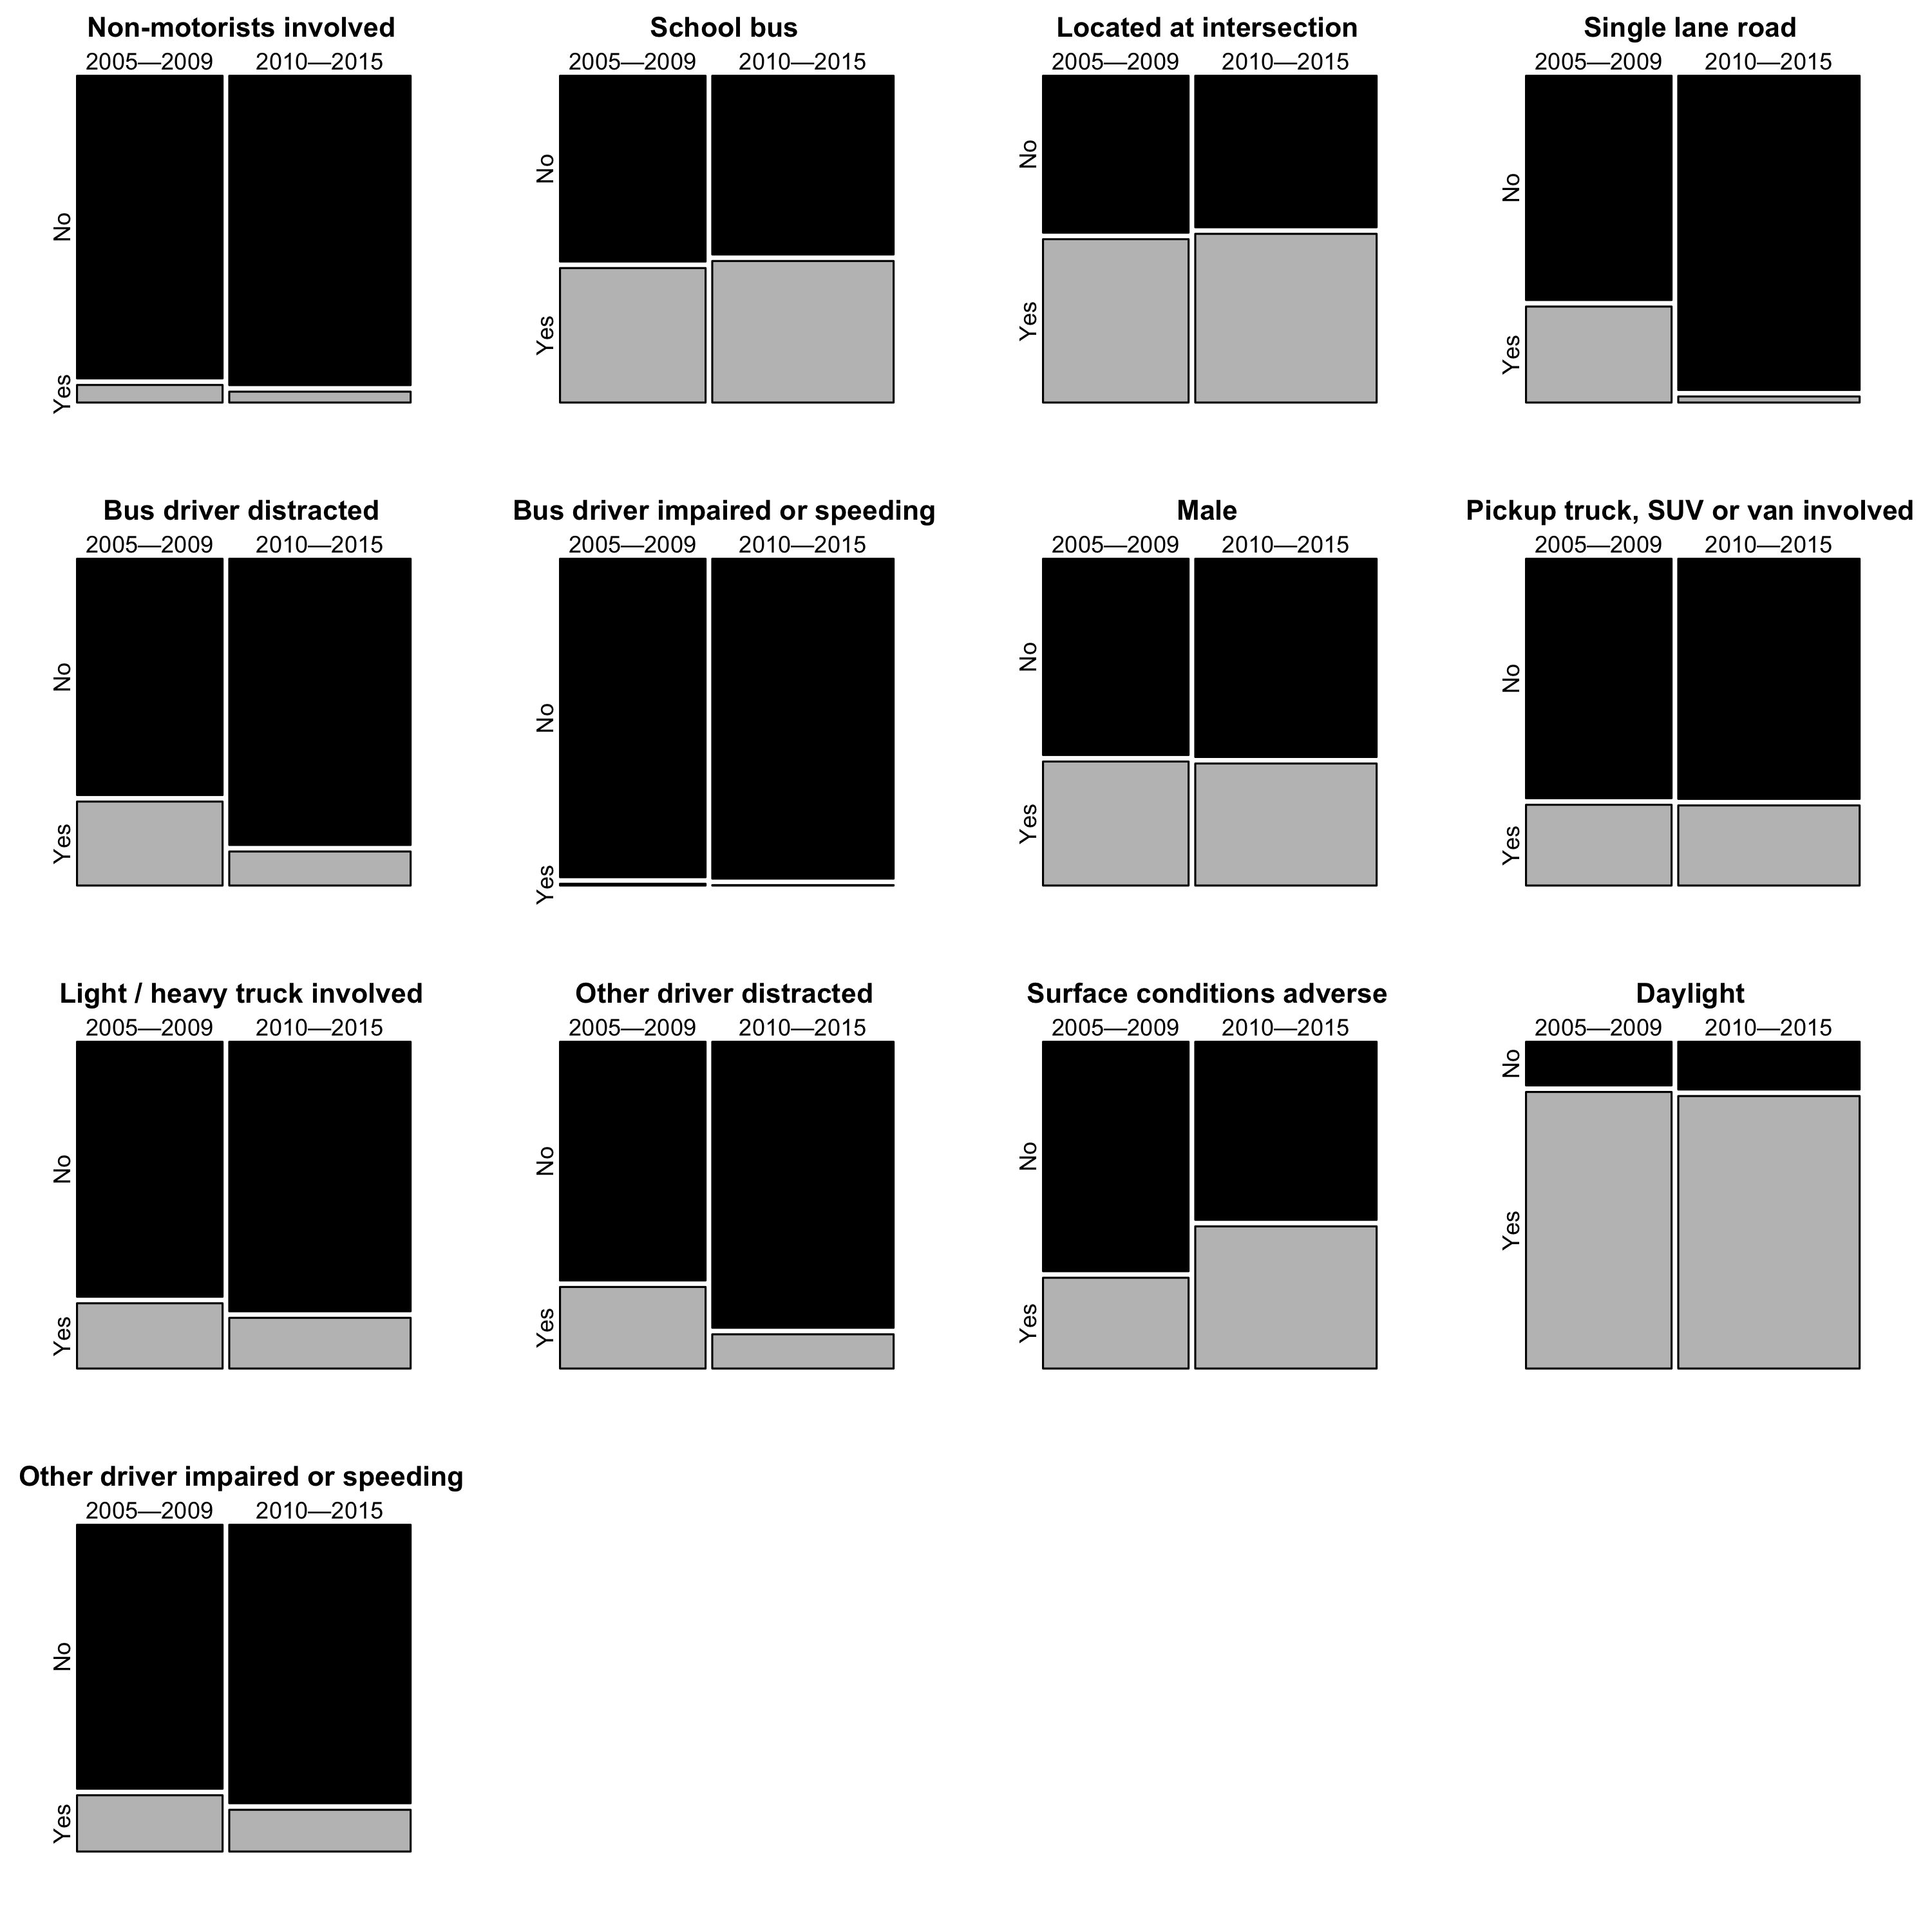
\includegraphics[width=\textwidth]{props.png}
%        \label{fig:props1}
%\end{figure}
%%%%%%%%%%%%%%%%%%%%%%%%%%%%%%%%%%%%%%%%%%%%%%%%%%%%%%%%%%%%%%%%%%%%%%%%%%%%%%%%%%%%%
%
%Figure \ref{fig:cat1} gives grouped bar plots for the categorical variables considered in the analysis. As these plots indicate, there are noticeable differences in the distribution of the variables for traffic control, critical event that made the crash imminent, and bus movement prior to the event. These variables seem to be distributed differently in the two time periods, information which is used in the clustering.
%%%%%%%%%%%%%%%%%%%%%%%%%%%%%%%%%%%%%%%%%%%%%%%%%%%%%%%%%%%%%%%%%%%%%%%%%%%%%%%%%%%%%
%\begin{figure}[t]
%        \caption{Grouped bar plots comparing the categorical response variables across the 2005--2009 and 2010--2015 datasets.}
%        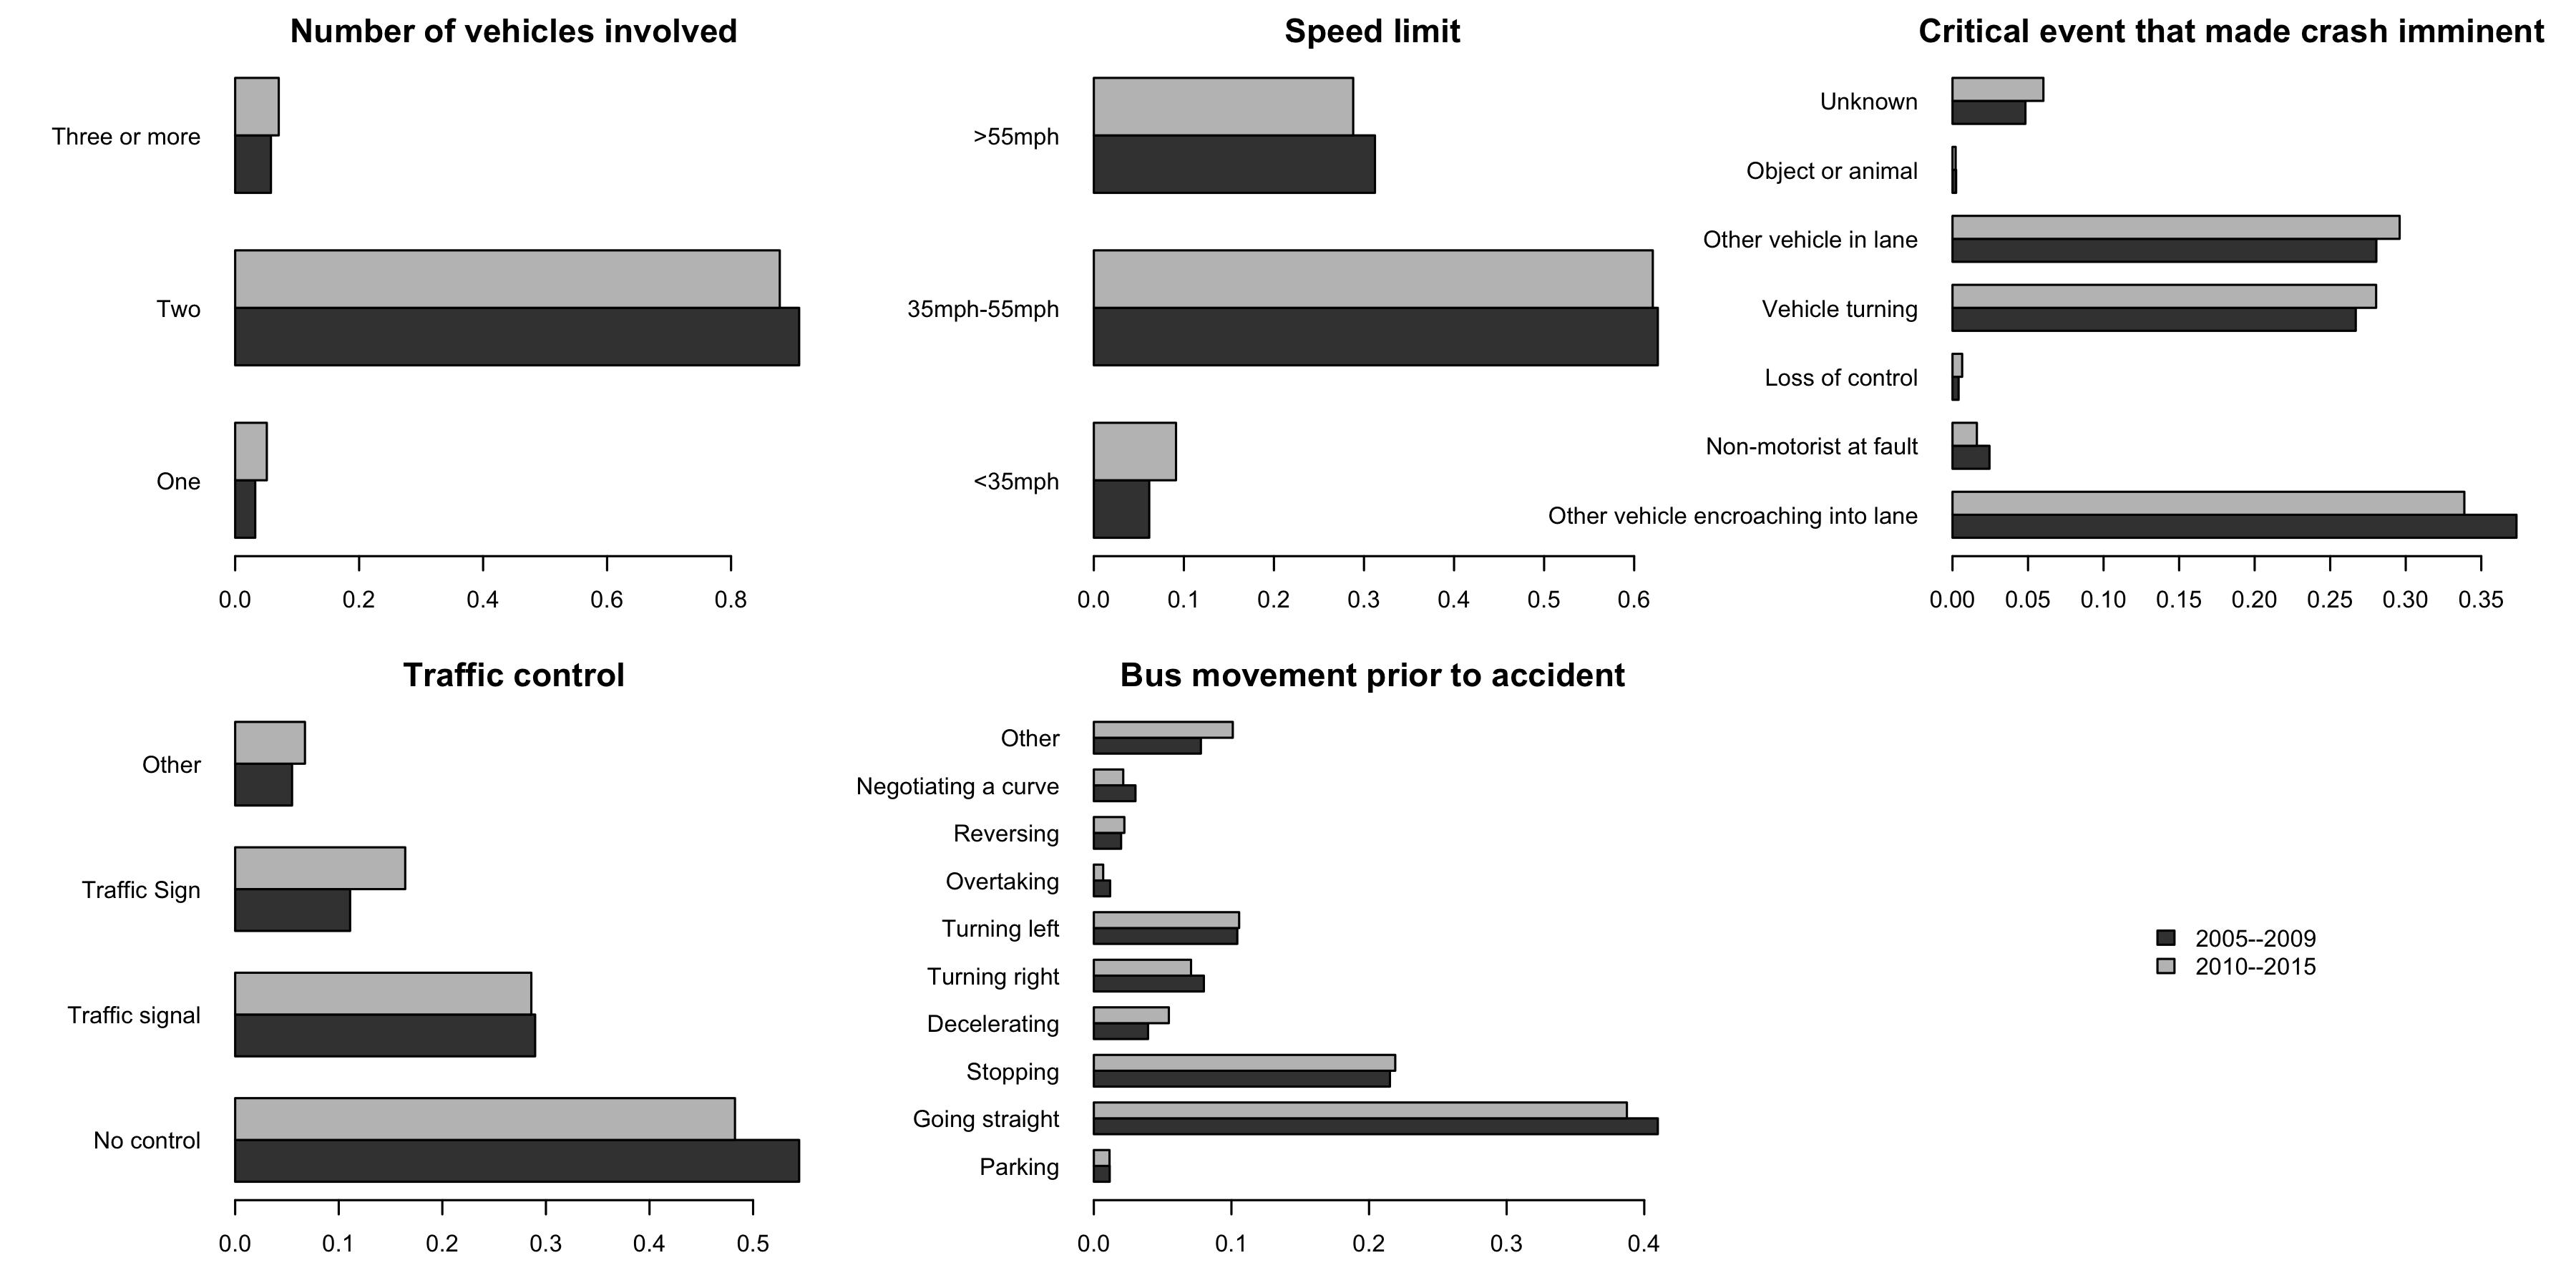
\includegraphics[width=\textwidth]{radar-bar.png}
%        \label{fig:cat1}
%\end{figure}
%%%%%%%%%%%%%%%%%%%%%%%%%%%%%%%%%%%%%%%%%%%%%%%%%%%%%%%%%%%%%%%%%%%%%%%%%%%%%%%%%%%%%

We chose a $20\times 20$ grid of neurons for the SOM clustering method, similar to \citet{prato2013bus}. The neural gas algorithm partitioned the data into four clusters, which we chose to optimally balance cluster homogeneity and differentiation. We used the R programming language \citep{r:r} to implement the two-stage clustering. We performed SOM using the package ``kohonen'' \citep{r:kohonen}, \citep{r:r} and we used ``cclust'' for the neural gas algorithm \citep{r:cclust}, \citep{r:r}.

Based on the results of the analysis, the four clusters in the \textbf{2005--2009 dataset} can be described as follows:

%%%%%%%%%%%%%%%%%%%%%%%%%%%%%%%%%%%%%%%%%%%%%%%%%%%%%%%%%%%%%%%%%%%%%%%%%%%%%%%%%%%%
\begin{figure}[t]
        %\centering
        \begin{subfigure}[t]{.5\textwidth}
%  \centering
                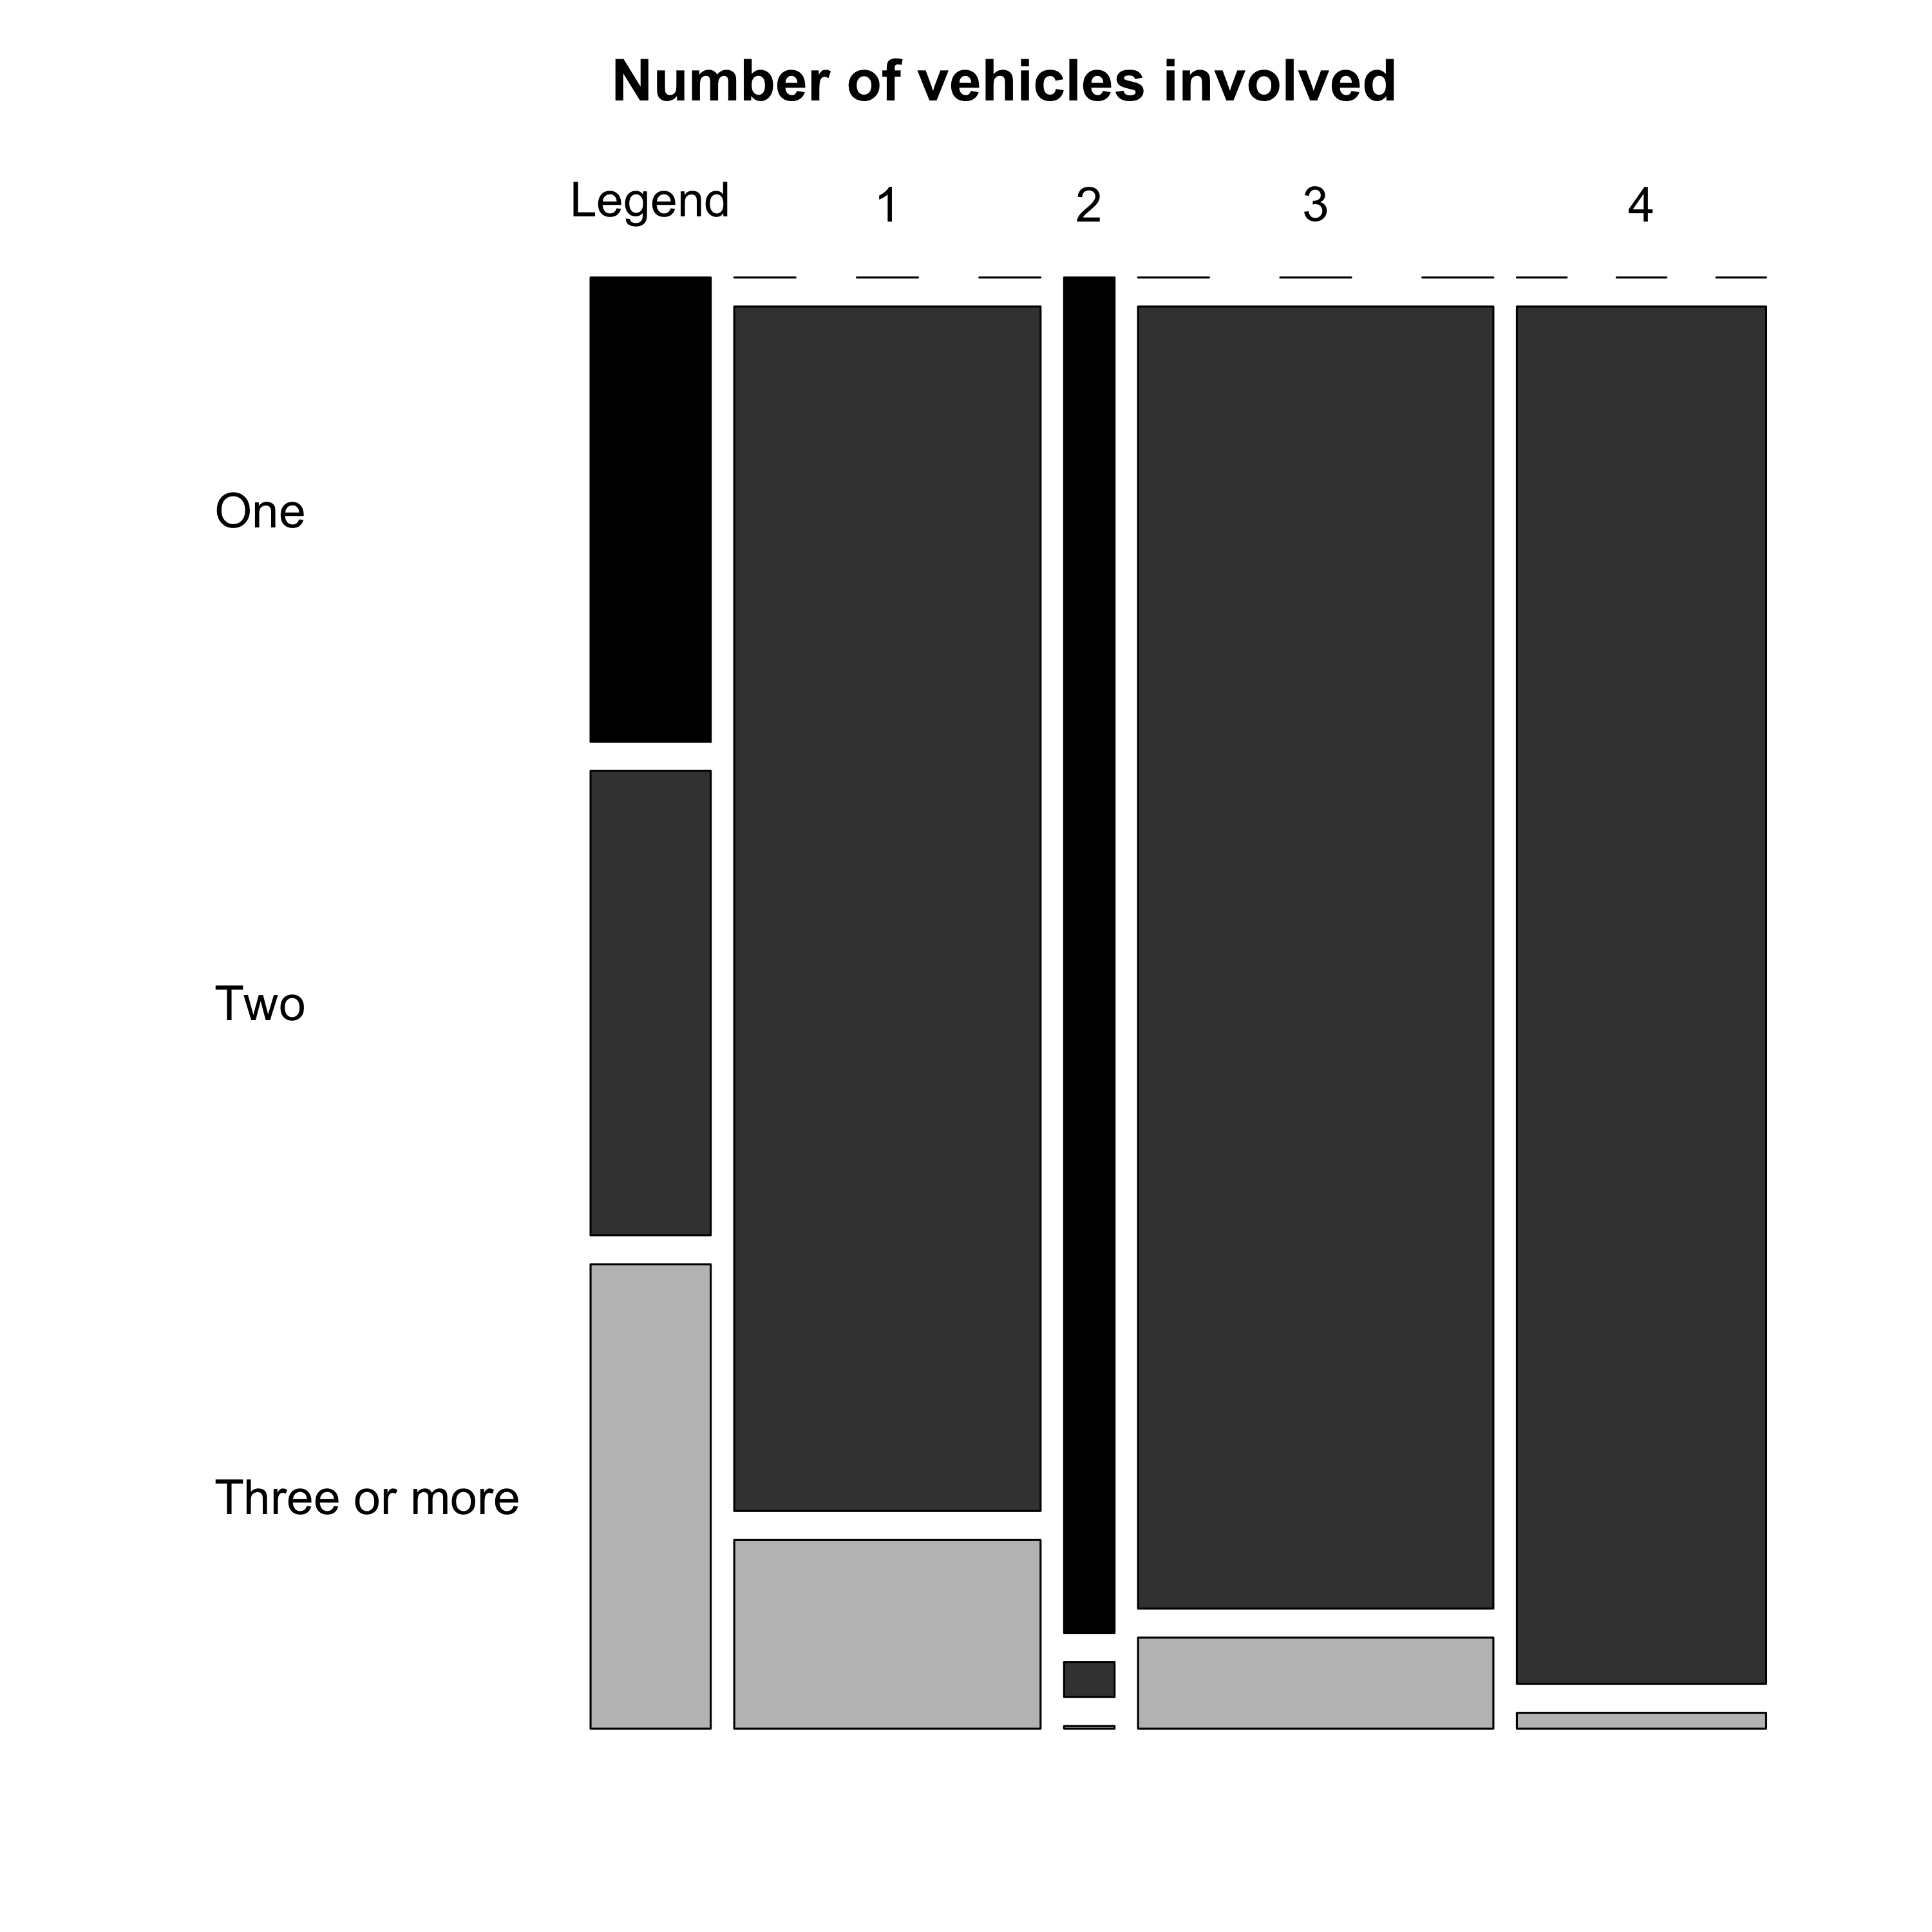
\includegraphics[width=1\linewidth]{veh_invl_0509.png}
                \caption{2005--2009}
        \end{subfigure}%
        \begin{subfigure}[t]{.5\textwidth}
%  \centering
                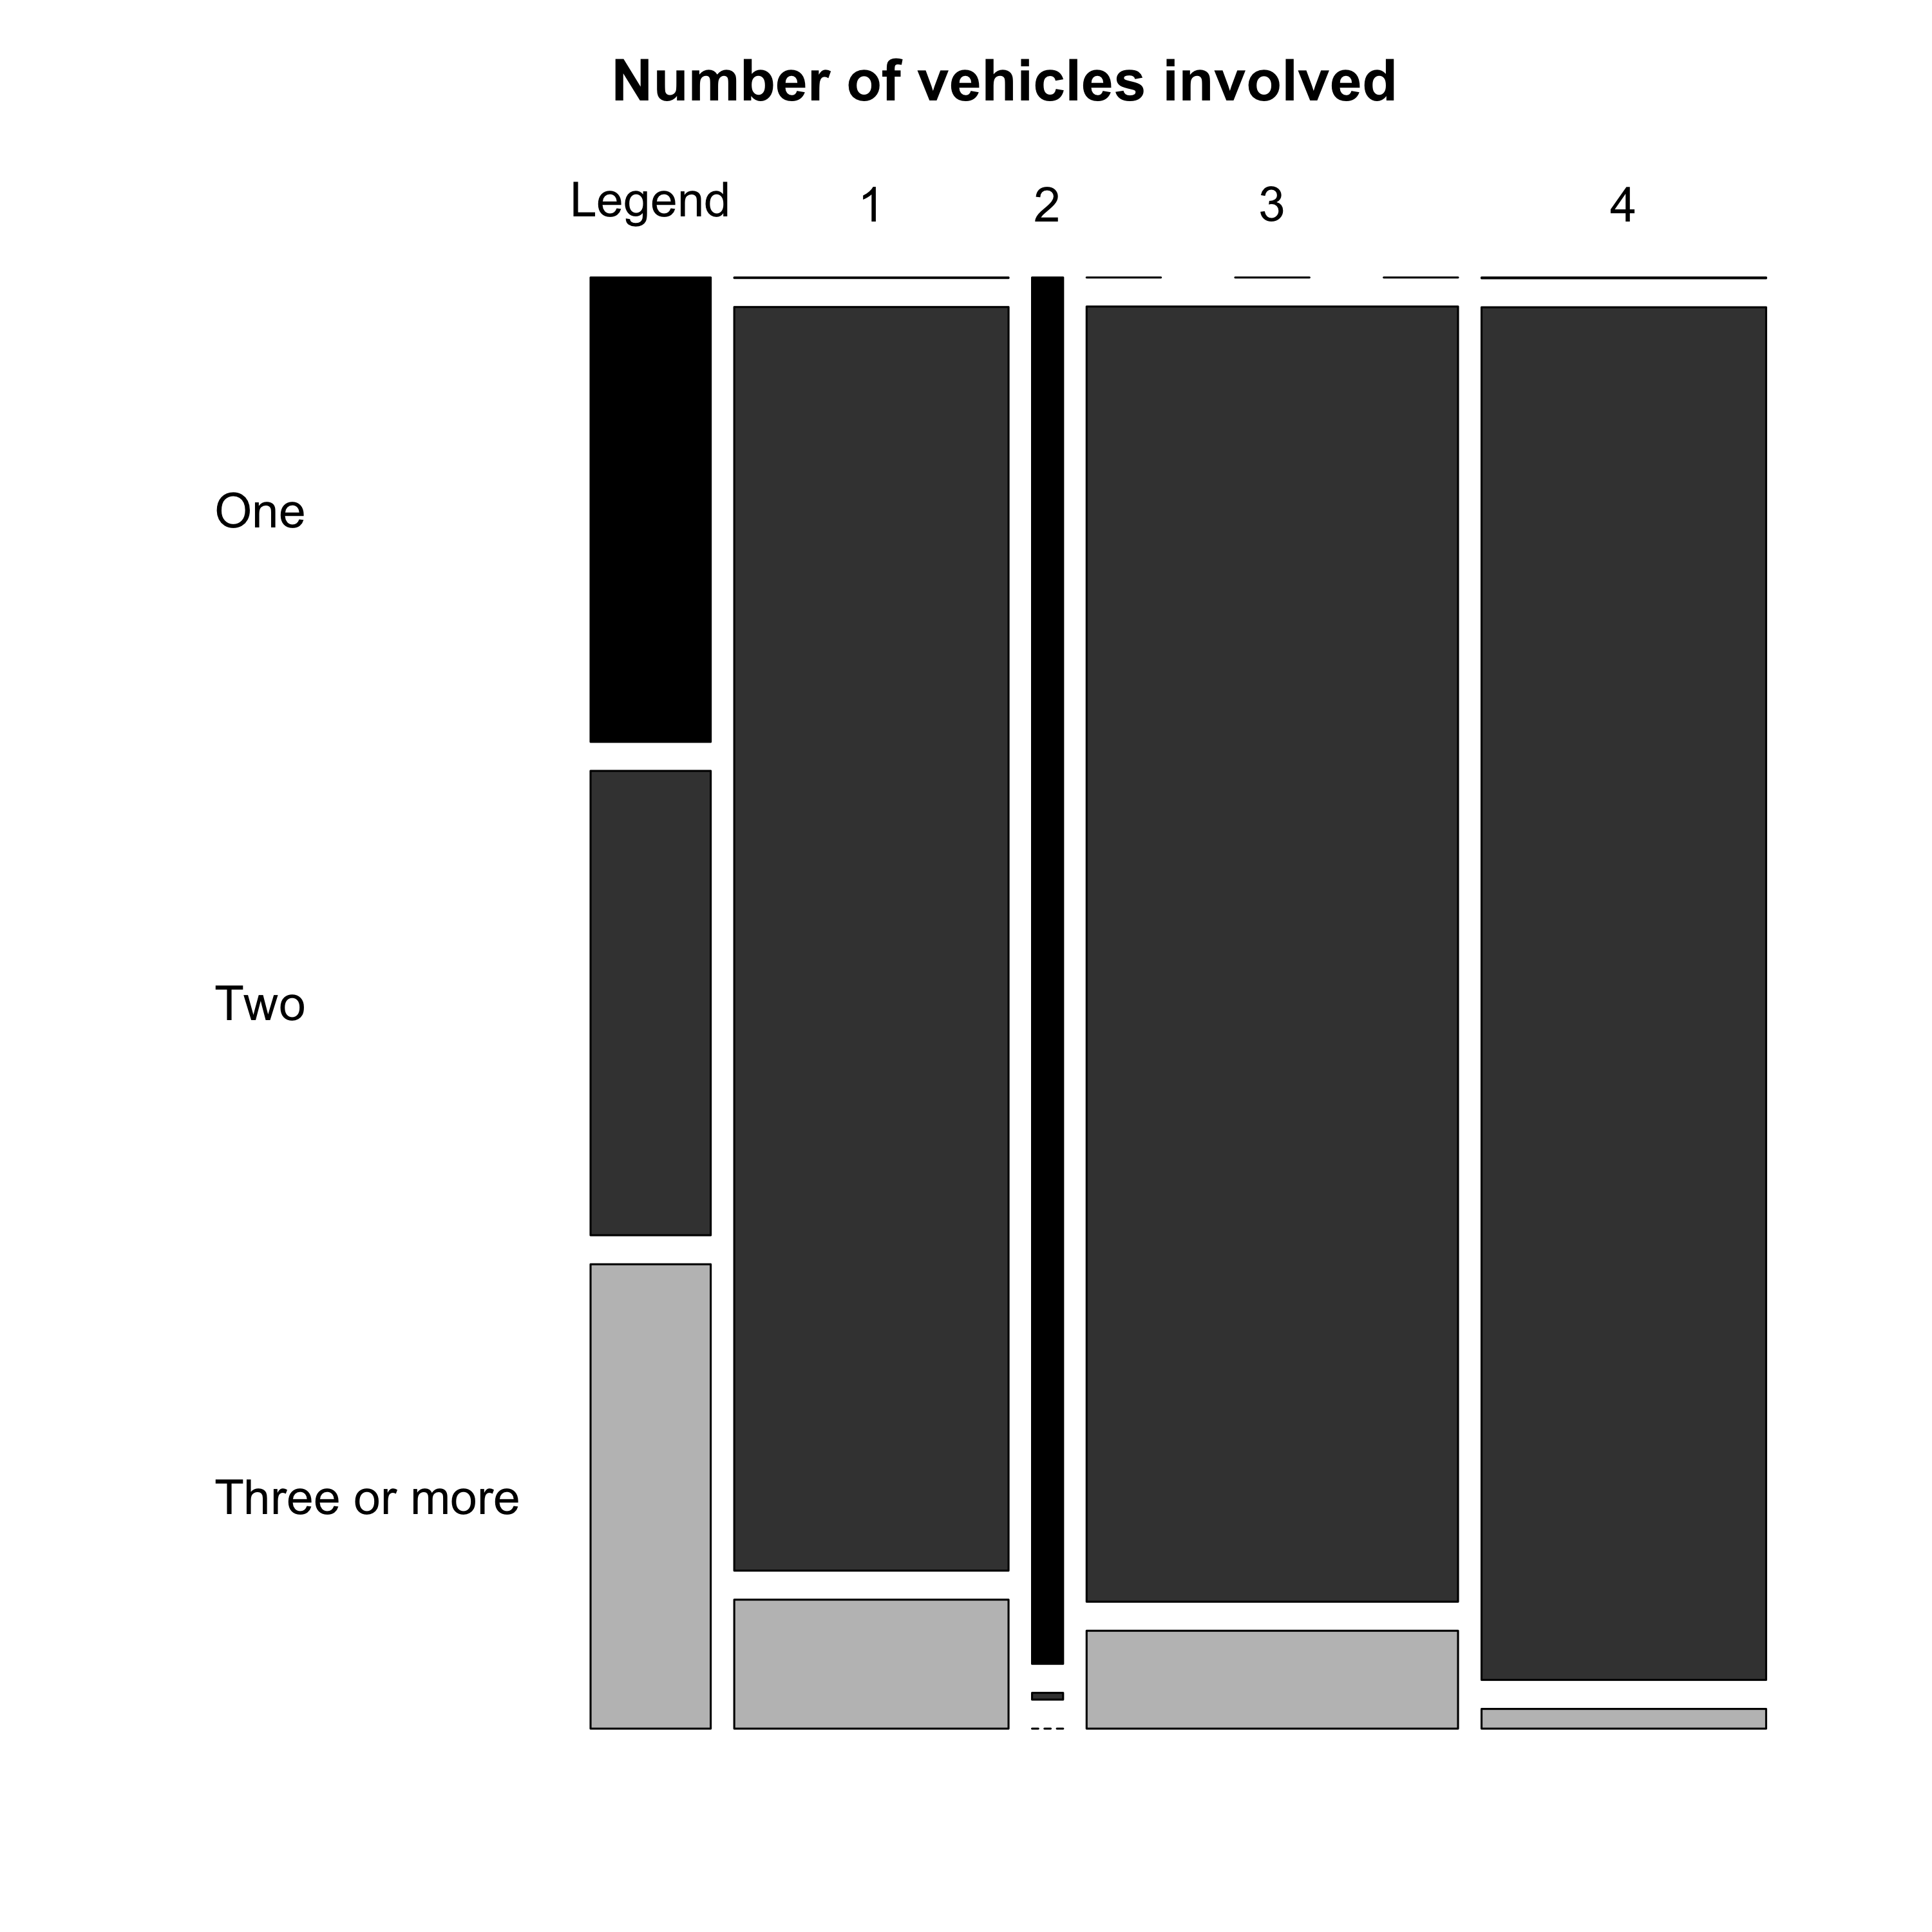
\includegraphics[width=1\linewidth]{veh_invl.png}
                \caption{2010--2015}
        \end{subfigure}
        \caption{Mosaic plots giving the breakdown of the variable ``number of vehicles involved in the accident'' for each of the four clusters.}
 \label{fig:clus10}
\end{figure}
%%%%%%%%%%%%%%%%%%%%%%%%%%%%%%%%%%%%%%%%%%%%%%%%%%%%%%%%%%%%%%%%%%%%%%%%%%%%%%%%%%%%

\noindent
\textbf{Cluster 1}: Single vehicle crashes involving non-motorists (100\%), (Figure \ref{fig:clus10} (a)) that happened when the bus was going straight (37.8\%), turning left (19.4\%) or trying to park (15.1\%) (Figure \ref{fig:clus4} (a)). There were two primary reasons for the crash: the bus turned (49.2\%), or the non-motorist (pedestrians, cyclists, bicyclists, etc.) was at fault (29\%) (Figure \ref{fig:clus12} (a)). In 35.8\% of the cases, the bus driver admitted to have been distracted. 40.8\% of the time, a school bus was involved. 4.7\% of the cases involved the non-motorist being impaired or under the influence. 42.9\% of the crashes happened at an intersection. 71.3\% of the crashes happened where the road had no traffic control, and in 14.3\% of the cases there was a traffic signal (Figure \ref{fig:clus8} (a)). 

\noindent
\textbf{Cluster 2}: Multi-vehicle crashes (93.1\% involving two vehicles) that occurred when the bus was going straight (64.2\%) or stopping (17.3\%). The crash was primarily due to the other vehicle encroaching into the bus' lane (92.1\%), implying that the crash was mainly the other driver's fault. In 19.7\% of the cases, the bus driver admitted to have been distracted, and 39.1\% of the time, a school bus was involved. Most of the crashes happened on roadways with moderate to high speed limits (61.5\% on roads with 35--55 MPH and 29.3\% on roads with greater than 55 MPH, Figure \ref{fig:clus6} (a)). For 25.6\% of the crashes, at least one of the other drivers involved was distracted, and 21.0\% of the cases involved at least one of the other drivers being impaired or under the influence. 50.3\% of the crashes happened at an intersection. 49.9\% of the crashes happened where the road had no traffic control, for 27.2\% of the cases there was a traffic signal, and in 18.1\% of the cases there was a traffic sign. 23.4\% of the cases involved a light or a heavy truck, and 23.1\% of the crashes involved an SUV, pickup truck, or van (Figure \ref{fig:clus2} (a)).

%%%%%%%%%%%%%%%%%%%%%%%%%%%%%%%%%%%%%%%%%%%%%%%%%%%%%%%%%%%%%%%%%%%%%%%%%%%%%%%%%%%%
\begin{figure}[t]
%\centering
        \begin{subfigure}{.5\textwidth}
%  \centering
                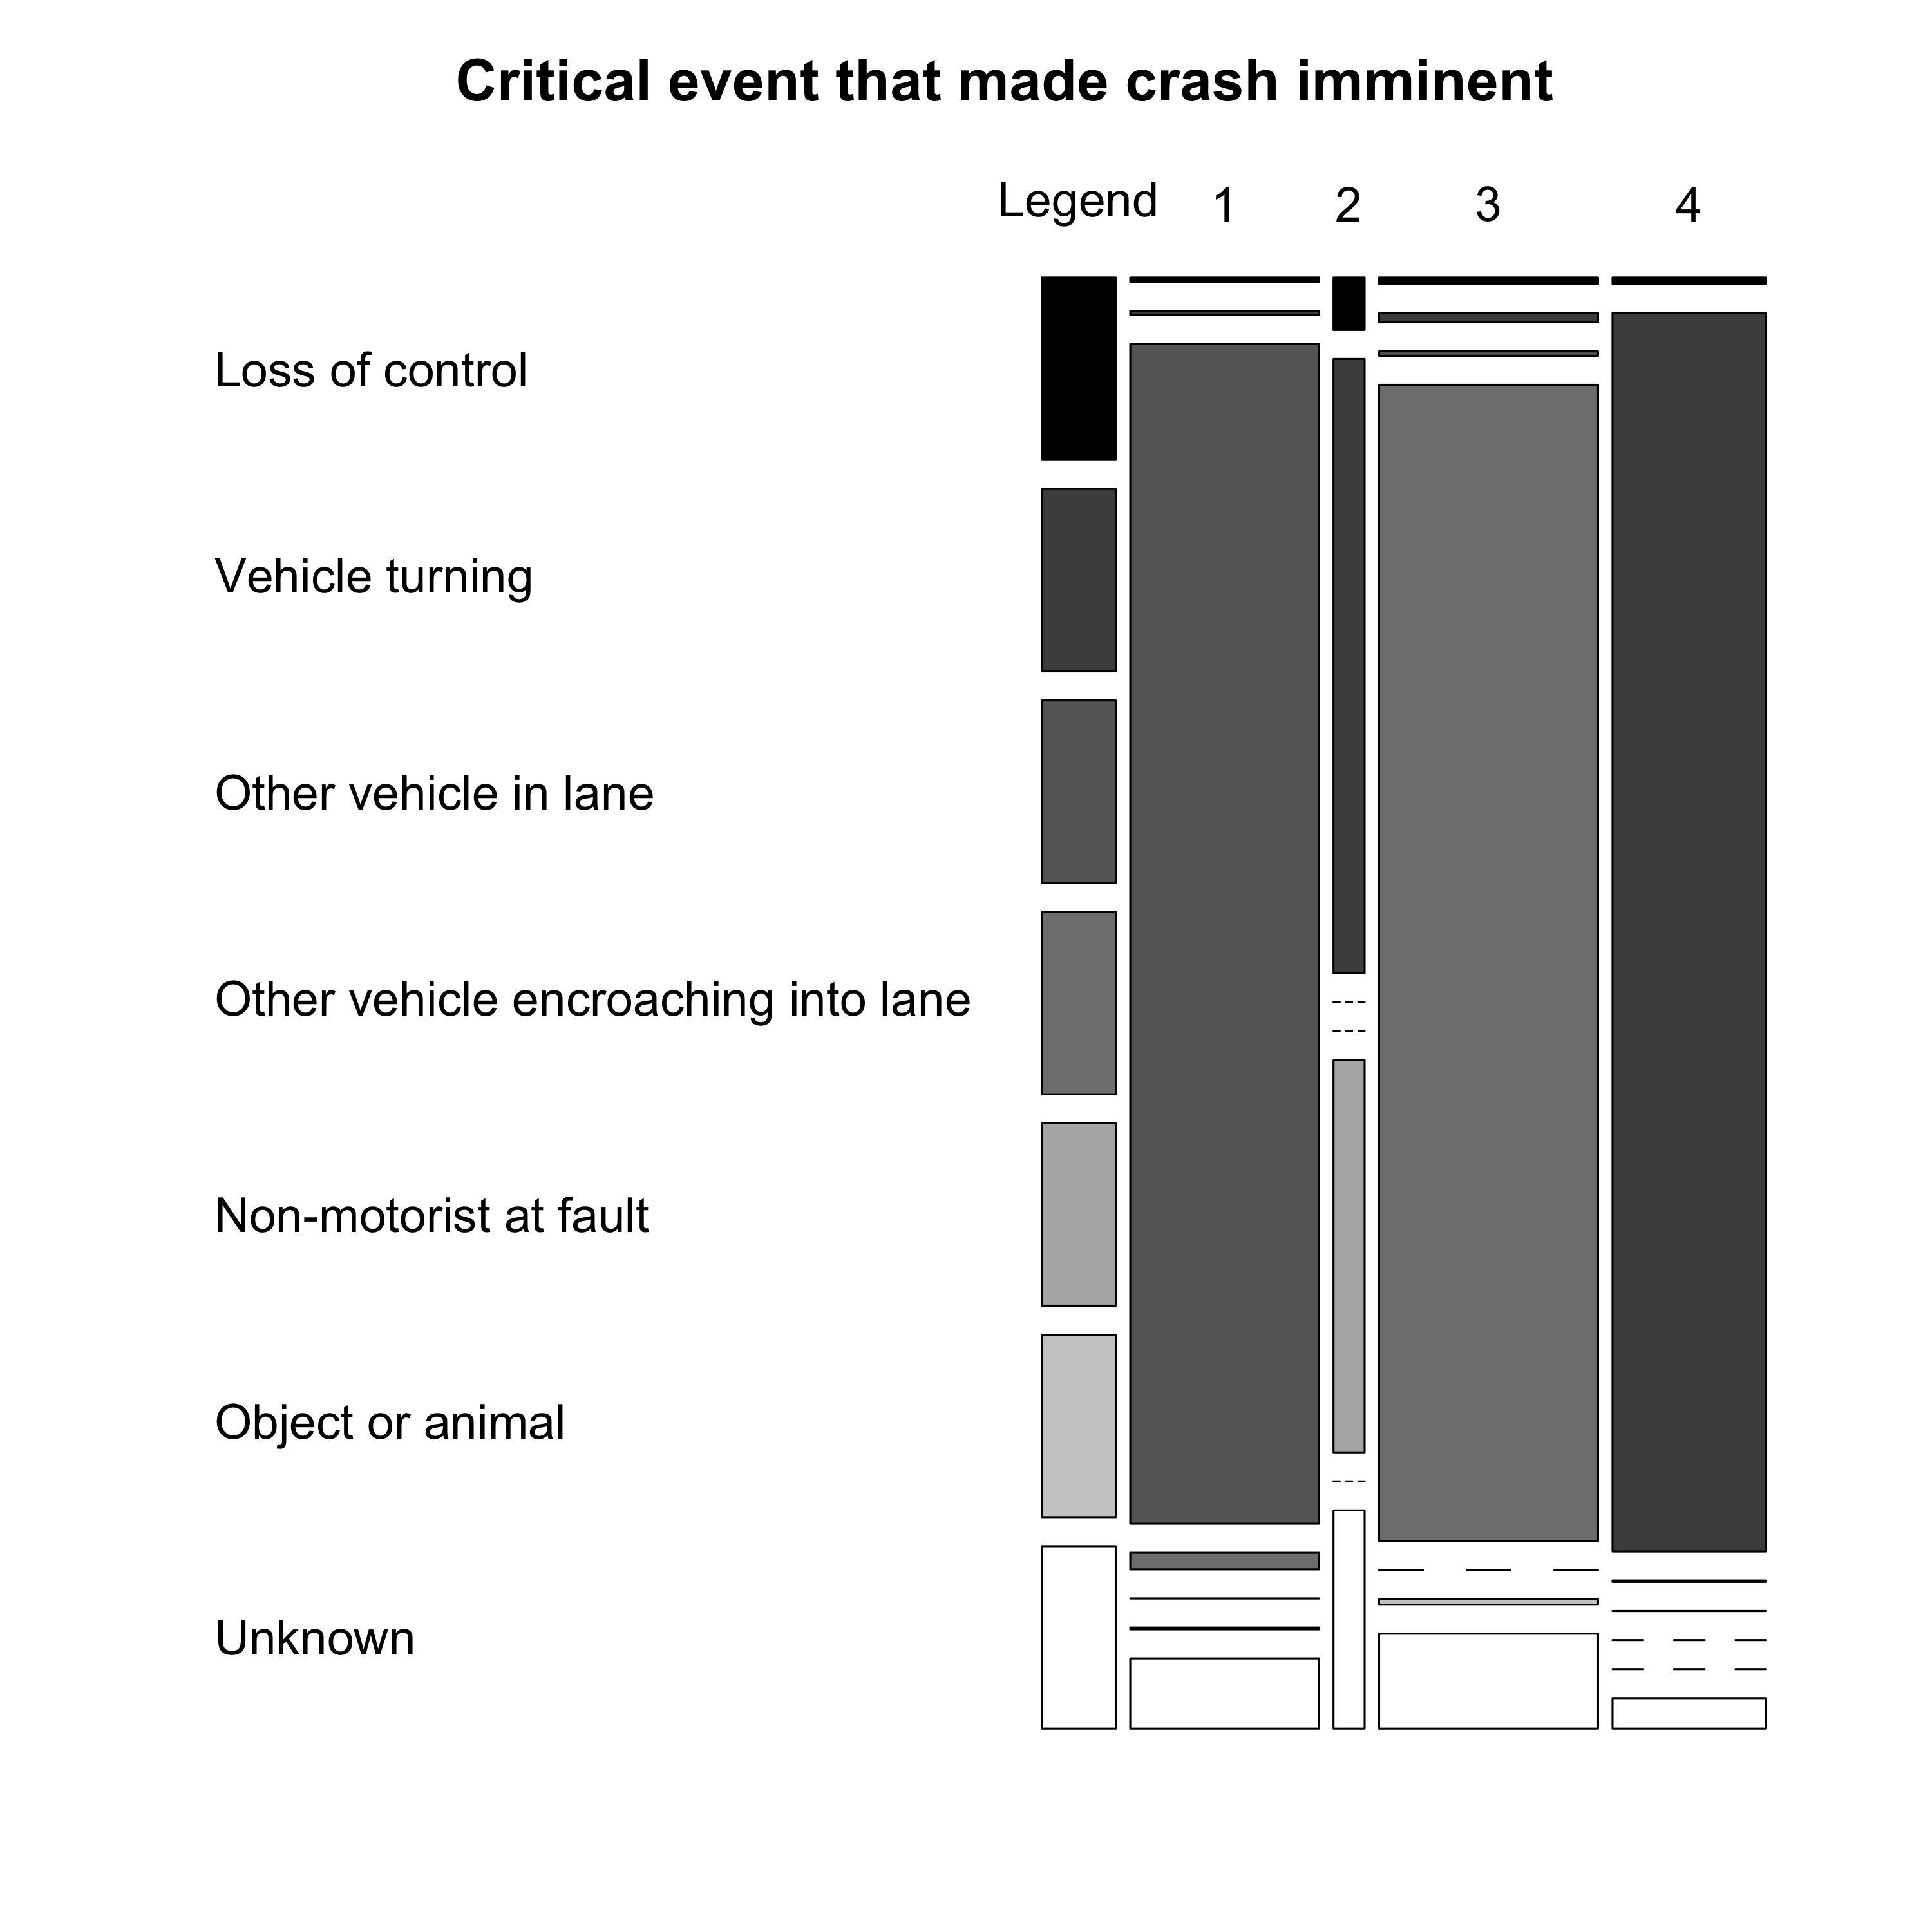
\includegraphics[width=1\linewidth]{crit_event_0509.png}
                \caption{2005--2009}
        \end{subfigure}%
        \begin{subfigure}{.5\textwidth}
%  \centering
                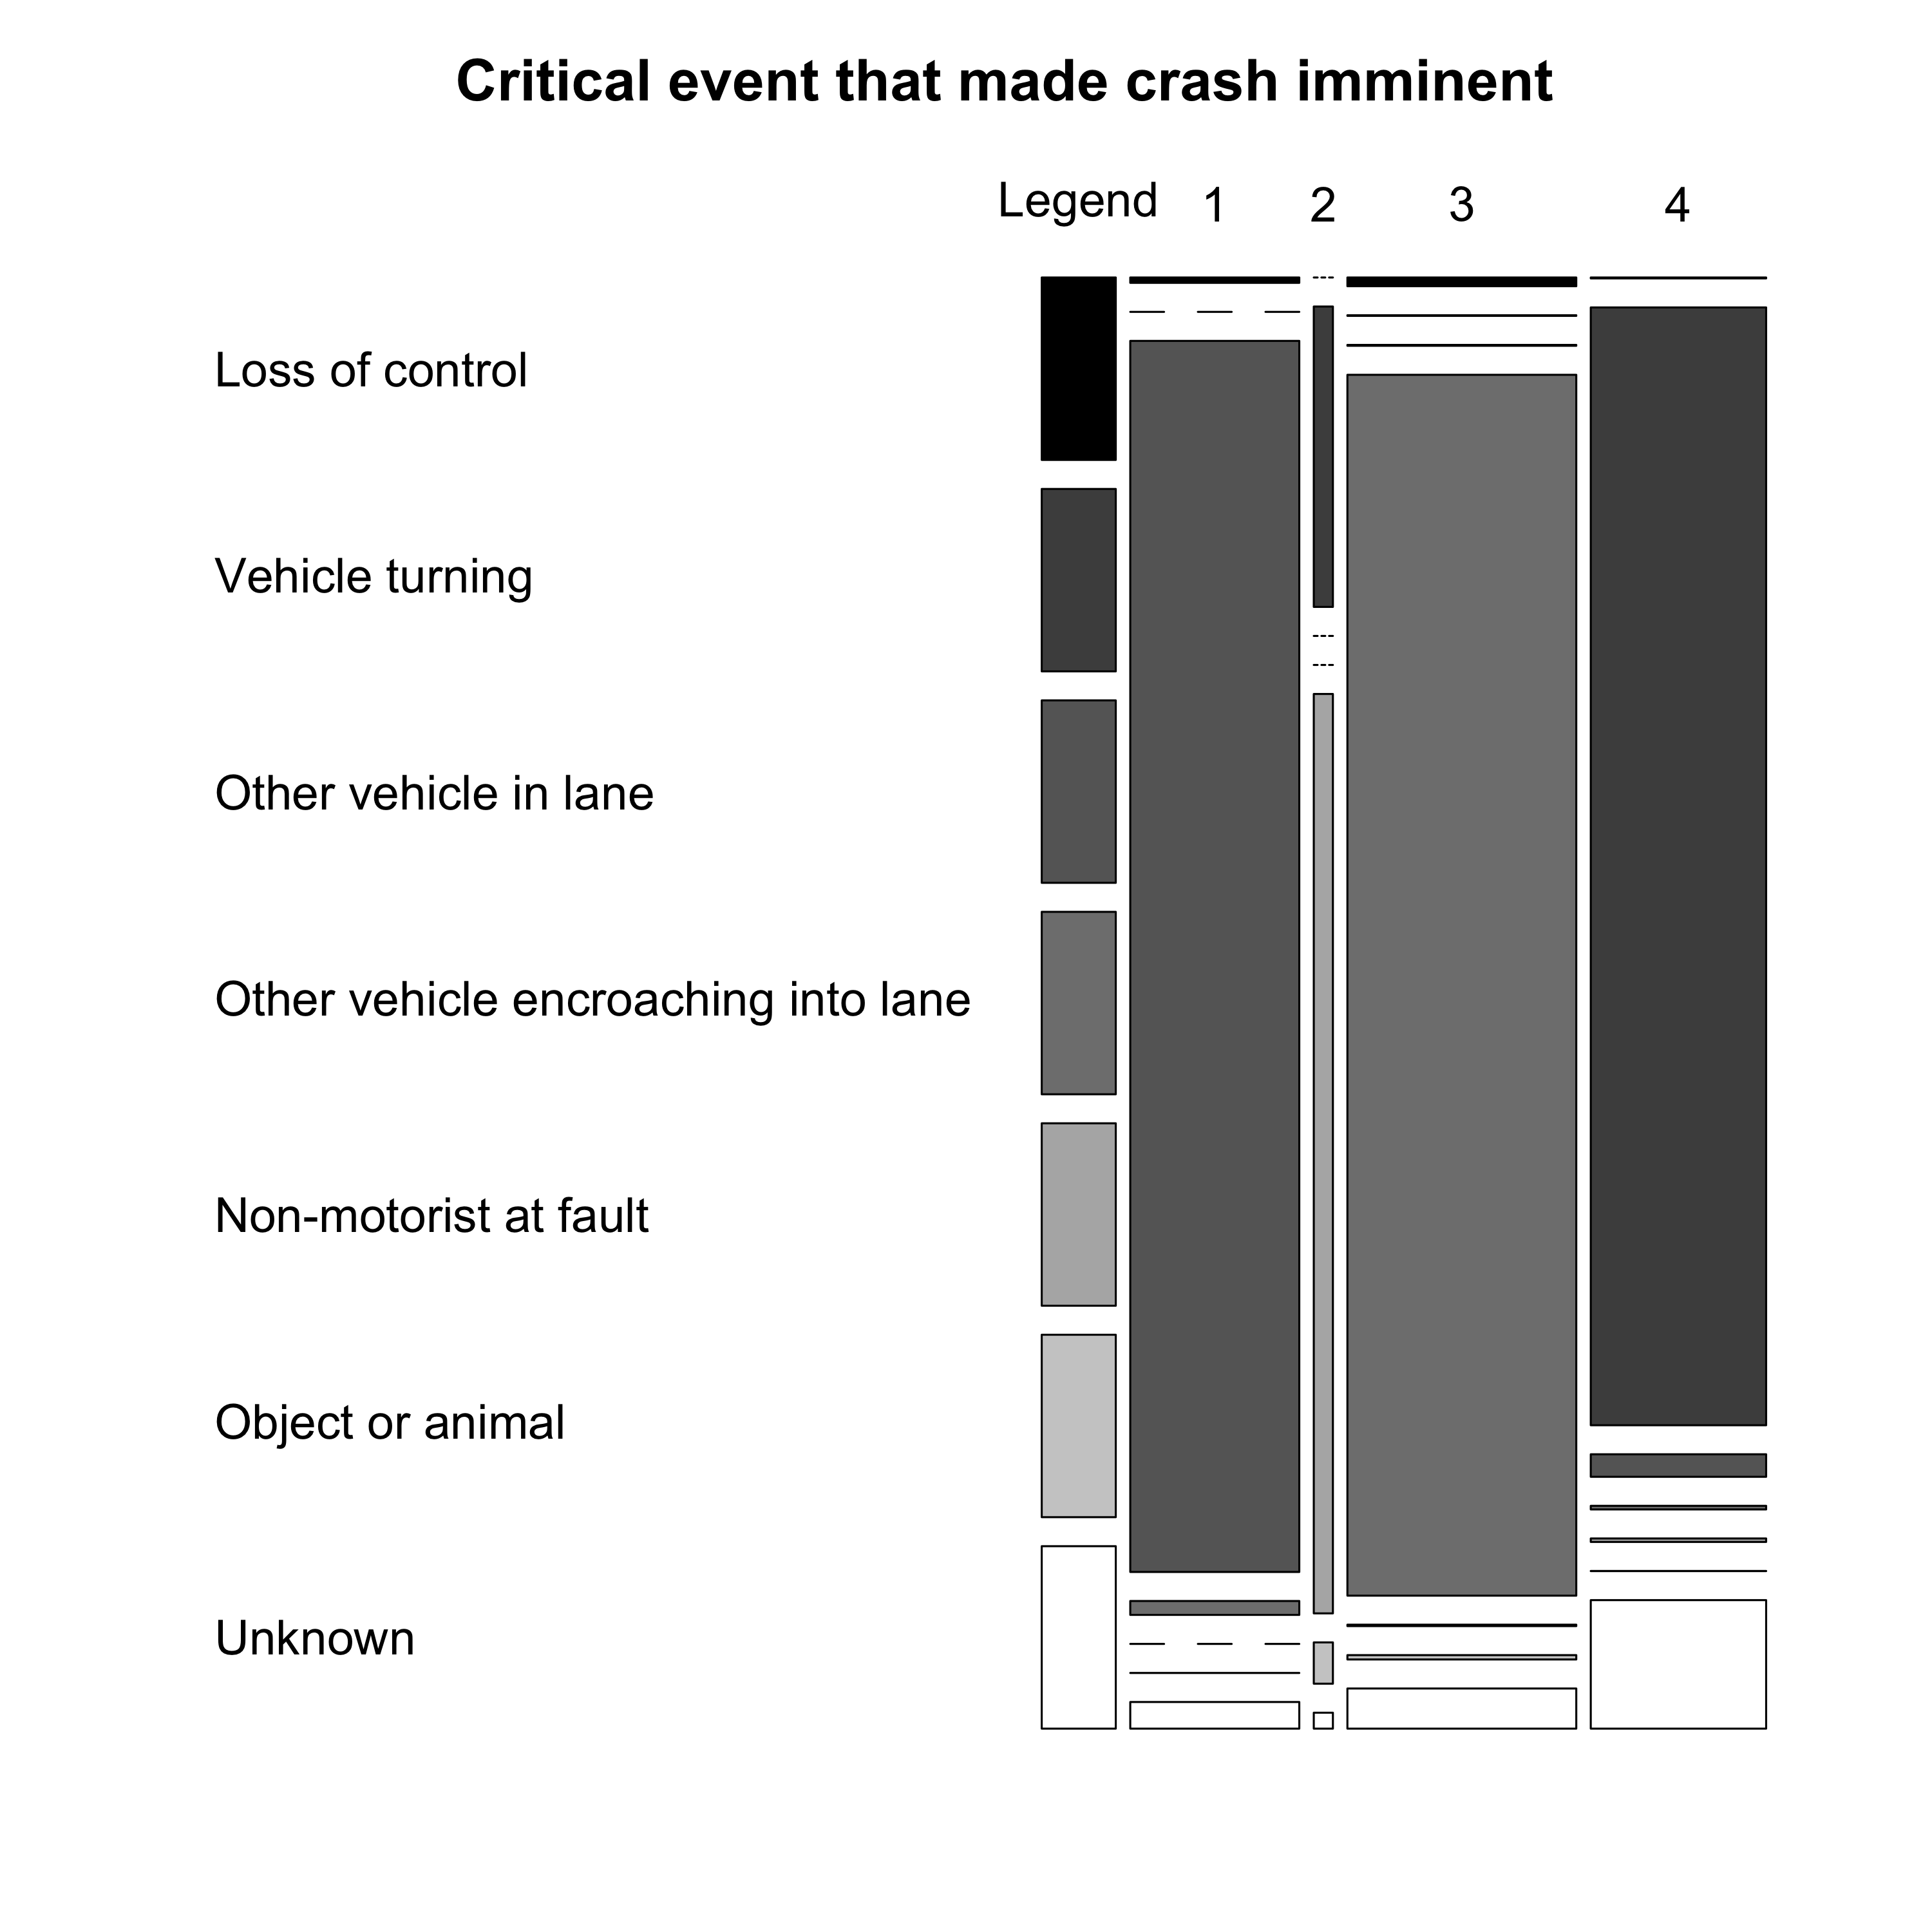
\includegraphics[width=1\linewidth]{crit_event.png}
                \caption{2010--2015}
        \end{subfigure}
        \caption{Mosaic plots giving the breakdown of the variable ``critical event that made the crash imminent'' for each of the four clusters.}
        \label{fig:clus12}
\end{figure}
%%%%%%%%%%%%%%%%%%%%%%%%%%%%%%%%%%%%%%%%%%%%%%%%%%%%%%%%%%%%%%%%%%%%%%%%%%%%%%%%%%%%

\noindent
\textbf{Cluster 3}:  Multi-vehicle crashes (86.1\% involving two vehicles, 13.9\% involving three or more vehicles), which happened largely due to the bus stopping (50.6\%), going straight (26.0\%) or decelerating (10.8\%). The cause of the crash was typically due to another vehicle being in the bus' lane (96.4\%). 27.1\% of the time, the bus driver was distracted. 51.7\% of the time, a school bus was involved. Most of the crashes happened during the daytime (89.9\%).
42.0\% of the time, the crash occurred at an intersection. In 31.0\% of the cases, the police found at least one driver of the other vehicles involved in the crash distracted and in 23.0\% of the cases, at least one of the other drivers was under the influence of alcohol, or drugs, or was impaired in some way. In 21.5\% of the cases, one of the other vehicles was a truck and in another 27.6\%, crashes involved an SUV, pickup truck, or van. 65.9\% of the crashes happened on roads with speed limit between 35--55 MPH, implying that these happened within a city or town and not on the highways.  48.7\% of the crashes happened where the road had no traffic control, and in 28.0\% of the cases, there was a traffic signal.
%%%%%%%%%%%%%%%%%%%%%%%%%%%%%%%%%%%%%%%%%%%%%%%%%%%%%%%%%%%%%%%%%%%%%%%%%%%%%%%%%%%%
\begin{figure}[t]
%\centering
        \begin{subfigure}{.5\textwidth}
%  \centering
                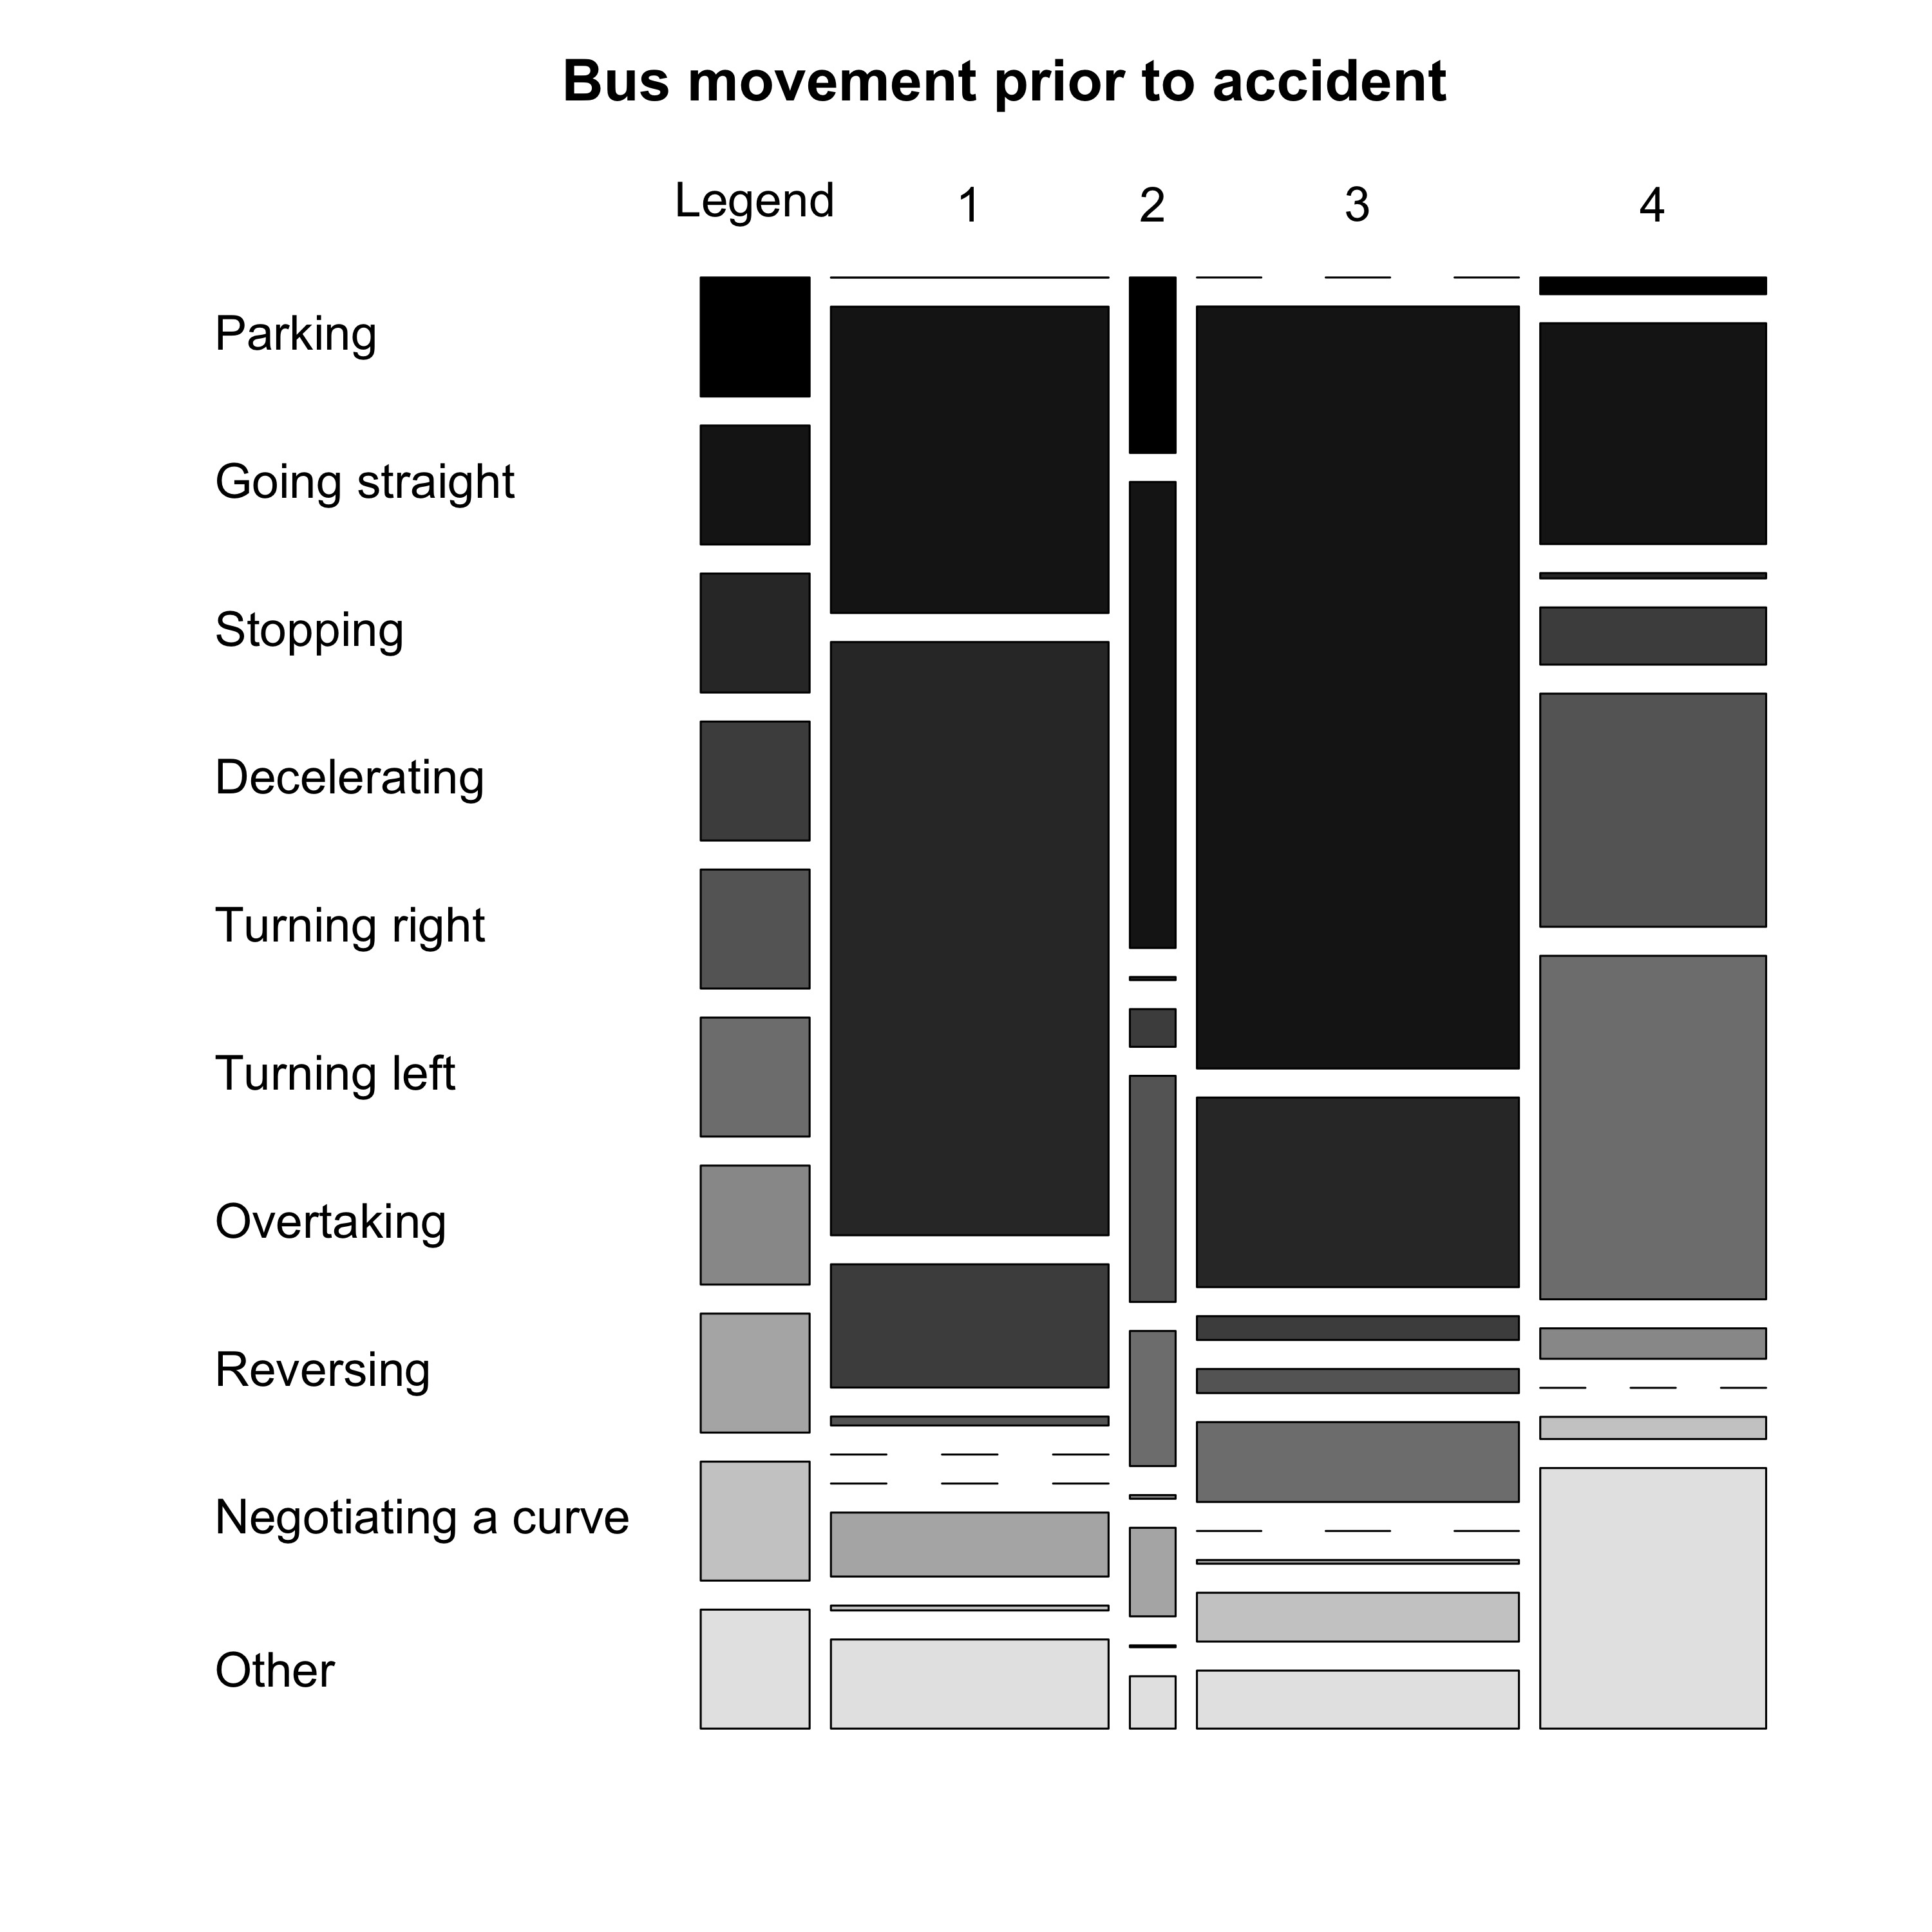
\includegraphics[width=1\linewidth]{bus_mov_0509.png}
                \caption{2005--2009}
        \end{subfigure}%
        \begin{subfigure}{.5\textwidth}
%  \centering
                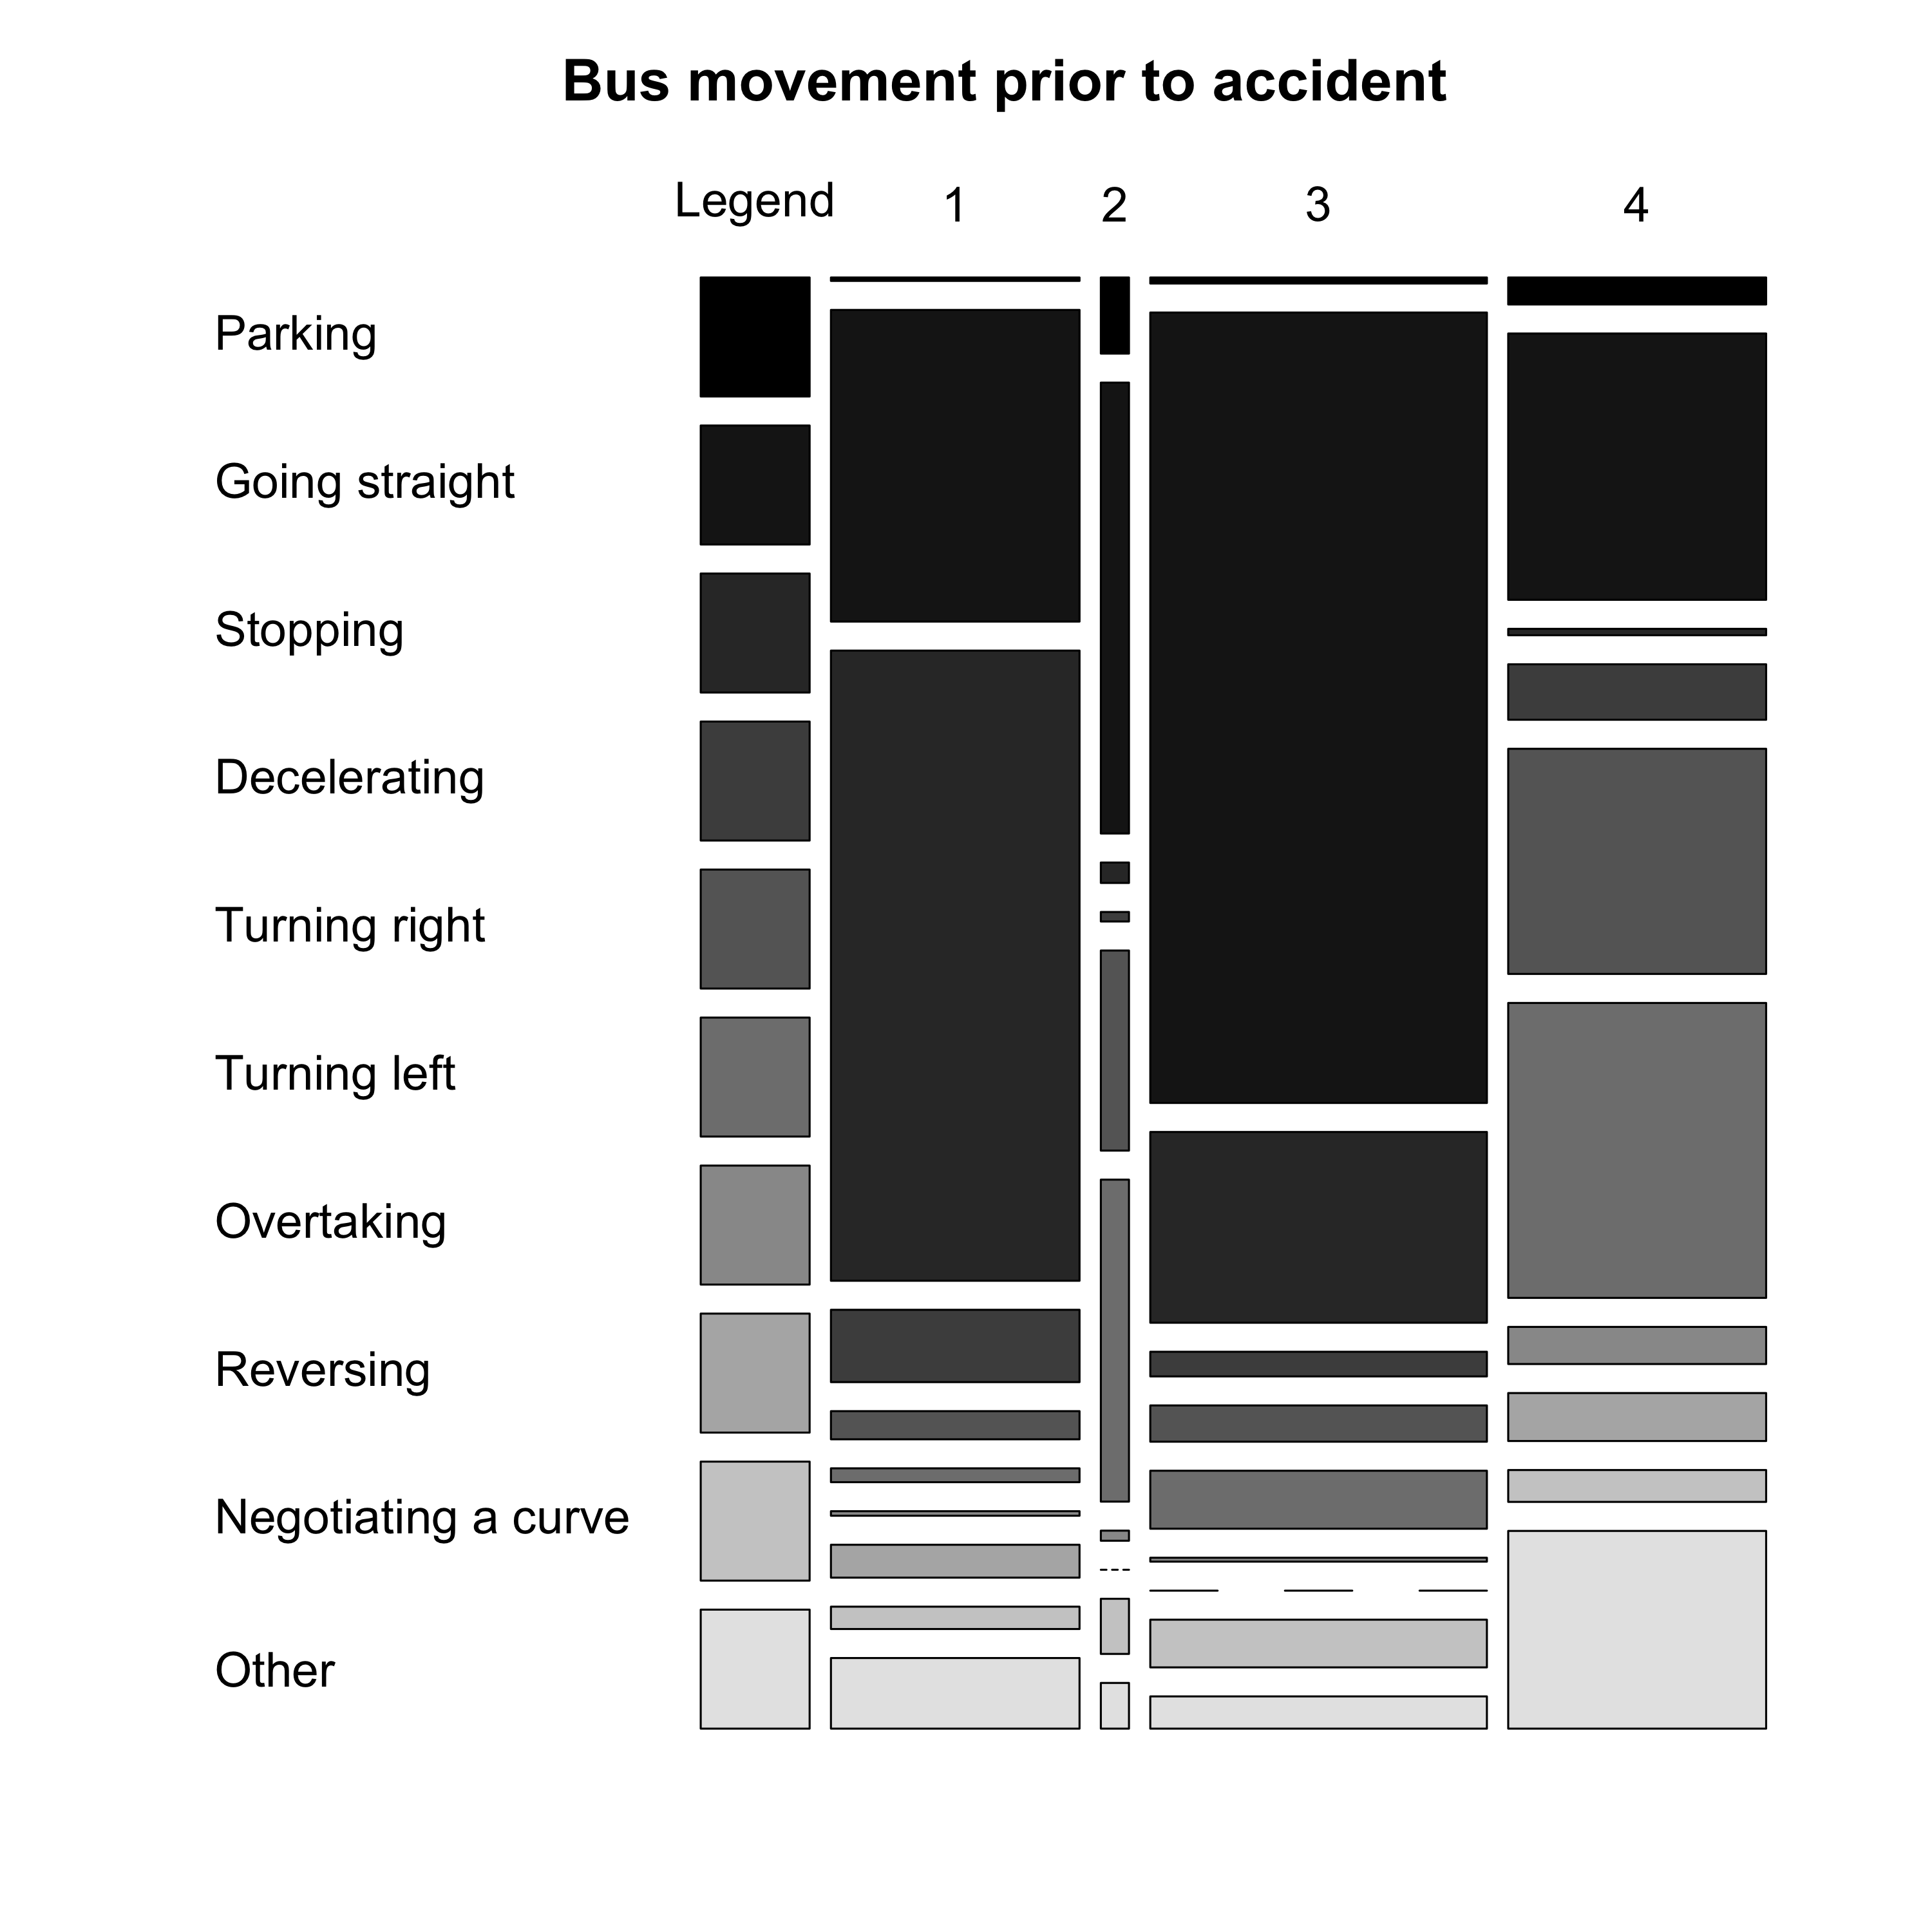
\includegraphics[width=1\linewidth]{bus_mov.png}
                \caption{2010--2015}
        \end{subfigure}
        \caption{Mosaic plots giving the breakdown of the variable ``bus movement prior to the crash'' for each of the four clusters.}
        \label{fig:clus4}
\end{figure} 
%%%%%%%%%%%%%%%%%%%%%%%%%%%%%%%%%%%%%%%%%%%%%%%%%%%%%%%%%%%%%%%%%%%%%%%%%%%%%%%%%%%%

\noindent
\textbf{Cluster 4}: Multi-vehicle crashes (98.9\% involving two vehicles) that happened when the bus was going straight (19.7\%), turning left (27.1\%) or making other movements such as passing/overtaking, merging, making a U-turn etc.   (20.5\%). The crash was primarily due to the bus trying to turn (90.7\%). In 32.1\% of the cases, the bus driver admitted to being distracted, and 35.4\% of the time, a school bus was involved. Most of the crashes happened on roadways with moderate to high speed limits (59.6\% on roads with 35--55 MPH and 33.8\% on roads with greater than 55 MPH). In only 4.9\% of the crashes was at least one of the other drivers involved distracted, and only 10.5\% of the cases involved at least one of the other drivers being impaired or under the influence. 63.0\% of the crashes happened at an intersection. 41.3\% of the crashes happened where the road had no traffic control, and in 33.6\% of the cases there was a traffic signal. 18.9\% of the cases involved a light or a heavy truck, and 29.9\% crashes involved an SUV, pickup truck, or van.

\noindent
Table \ref{table:tax1} summarizes the characteristics of the 2005--2009 bus crash clusters. 
%\begin{table}[H]
%\centering
%\resizebox{\textwidth}{!}{%
%\begin{tabular}{lllll}
%\rowcolor[HTML]{C0C0C0} 
%\multicolumn{1}{c}{\cellcolor[HTML]{C0C0C0}\textbf{Attribute}} & \multicolumn{1}{c}{\cellcolor[HTML]{C0C0C0}\textbf{Cluster 1}} & \multicolumn{1}{c}{\cellcolor[HTML]{C0C0C0}\textbf{Cluster 2}} & \multicolumn{1}{c}{\cellcolor[HTML]{C0C0C0}\textbf{Cluster 3}} & \multicolumn{1}{c}{\cellcolor[HTML]{C0C0C0}\textbf{Cluster 4}} \\
%\begin{tabular}[c]{@{}l@{}}Single vs. Multiple vehicles\\ (\textgreater85\%)\end{tabular} & Multiple & {\color[HTML]{9A0000} Single} & Multiple & Multiple \\
%Non-motorist involvement & 0.1\% & {\color[HTML]{680100} 99.5\%} & 0.4\% & 0\% \\
%Bus movement prior to crash & {\color[HTML]{9A0000} \begin{tabular}[c]{@{}l@{}}Stopping \\ (49.8\%)\end{tabular}} & {\color[HTML]{333333} \begin{tabular}[c]{@{}l@{}}Parking (14.7\%),\\ Going straight \\ (39.2\%), turning \\ left (19\%)\end{tabular}} & \begin{tabular}[c]{@{}l@{}}Going straight\\ (64\%), \\ stopping \\ (15.9\%)\end{tabular} & \begin{tabular}[c]{@{}l@{}}Turning left\\ (19.6\%), \\ overtaking \\ (28.9\%), \\ other (21.9\%)\end{tabular} \\
%\begin{tabular}[c]{@{}l@{}}Critical event that made the \\ crash imminent\end{tabular} & \begin{tabular}[c]{@{}l@{}}In another \\ vehicle's \\ lane (92.3\%)\end{tabular} & \begin{tabular}[c]{@{}l@{}}Vehicle turning\\ (48.1\%), non-\\ motorist \\ encroaching into\\ lane (30.7\%)\end{tabular} & \begin{tabular}[c]{@{}l@{}}Encroaching\\ in another \\ vehicle's \\ lane (90.5\%)\end{tabular} & \begin{tabular}[c]{@{}l@{}}Vehicle \\ turning \\ (96.9\%)\end{tabular} \\ 
%Bus driver distracted & 27.4\% & 33.9\% & 20.2\% & 31.8\% \\ \\
%\begin{tabular}[c]{@{}l@{}}Other vehicle's driver or the \\ non-motorist charged with \\ alcohol/drug/impairment \\ related offense\end{tabular} & 22.1\% & {\color[HTML]{9A0000} 4.7\%} & 20.5\% & 10.5\% \\
%Was a school bus involved? & {\color[HTML]{9A0000} 51.8\%} & 39.8\% & 39.9\% & 32.2\% \\ \\
%\begin{tabular}[c]{@{}l@{}}Daylight condition - was there\\ sufficient light?\end{tabular} & 90.1\% & 89.5\% & 86.1\% & 81.4\% \\ \\
%\begin{tabular}[c]{@{}l@{}}Did the accident happen at an\\ intersection?\end{tabular} & 40.8\% & 44.3\% & 49.6\% & {\color[HTML]{9A0000} 66.9\%} \\ \\
%Bus driver (male)? & 56.9\% & 55.8\% & 62.7\% & 65.7\% \\ \\
%Light/ heavy truck involvement & 21.6\% & {\color[HTML]{9A0000} 0.1\%} & 22.5\% & 19.9\% \\ \\
%\begin{tabular}[c]{@{}l@{}}Was the other driver/ \\ non motorist distracted?\end{tabular} & 30.6\% & {\color[HTML]{9A0000} 100\%} & 24.9\% & {\color[HTML]{9A0000} 4.9\%} \\ \\
%\begin{tabular}[c]{@{}l@{}}Was there a pick-up truck/ van/\\ SUV involved?\end{tabular} & 28.4\% & 24.8\% & 27.1\% & {\color[HTML]{9A0000} 0\%} \\ \\
%Single lane vs. multiple lanes & {\color[HTML]{9A0000} 22.4\%} & 35.3\% & 31.1\% & 36.7\%
%\end{tabular}%
%}
%\caption{Taxonomy of crashes 2005 - 2009}
%\label{table: tax1}
%\end{table}
%%%%%%%%%%%%%%%%%%%%%%%%%%%%%%%%%%%%%%%%%%%%%%%%%%%%%%%%%%%%%%%%%%%%%%%%%%%%%%%%%%%%
\begin{figure}[t]
%\centering
        \begin{subfigure}{.5\textwidth}
%  \centering
                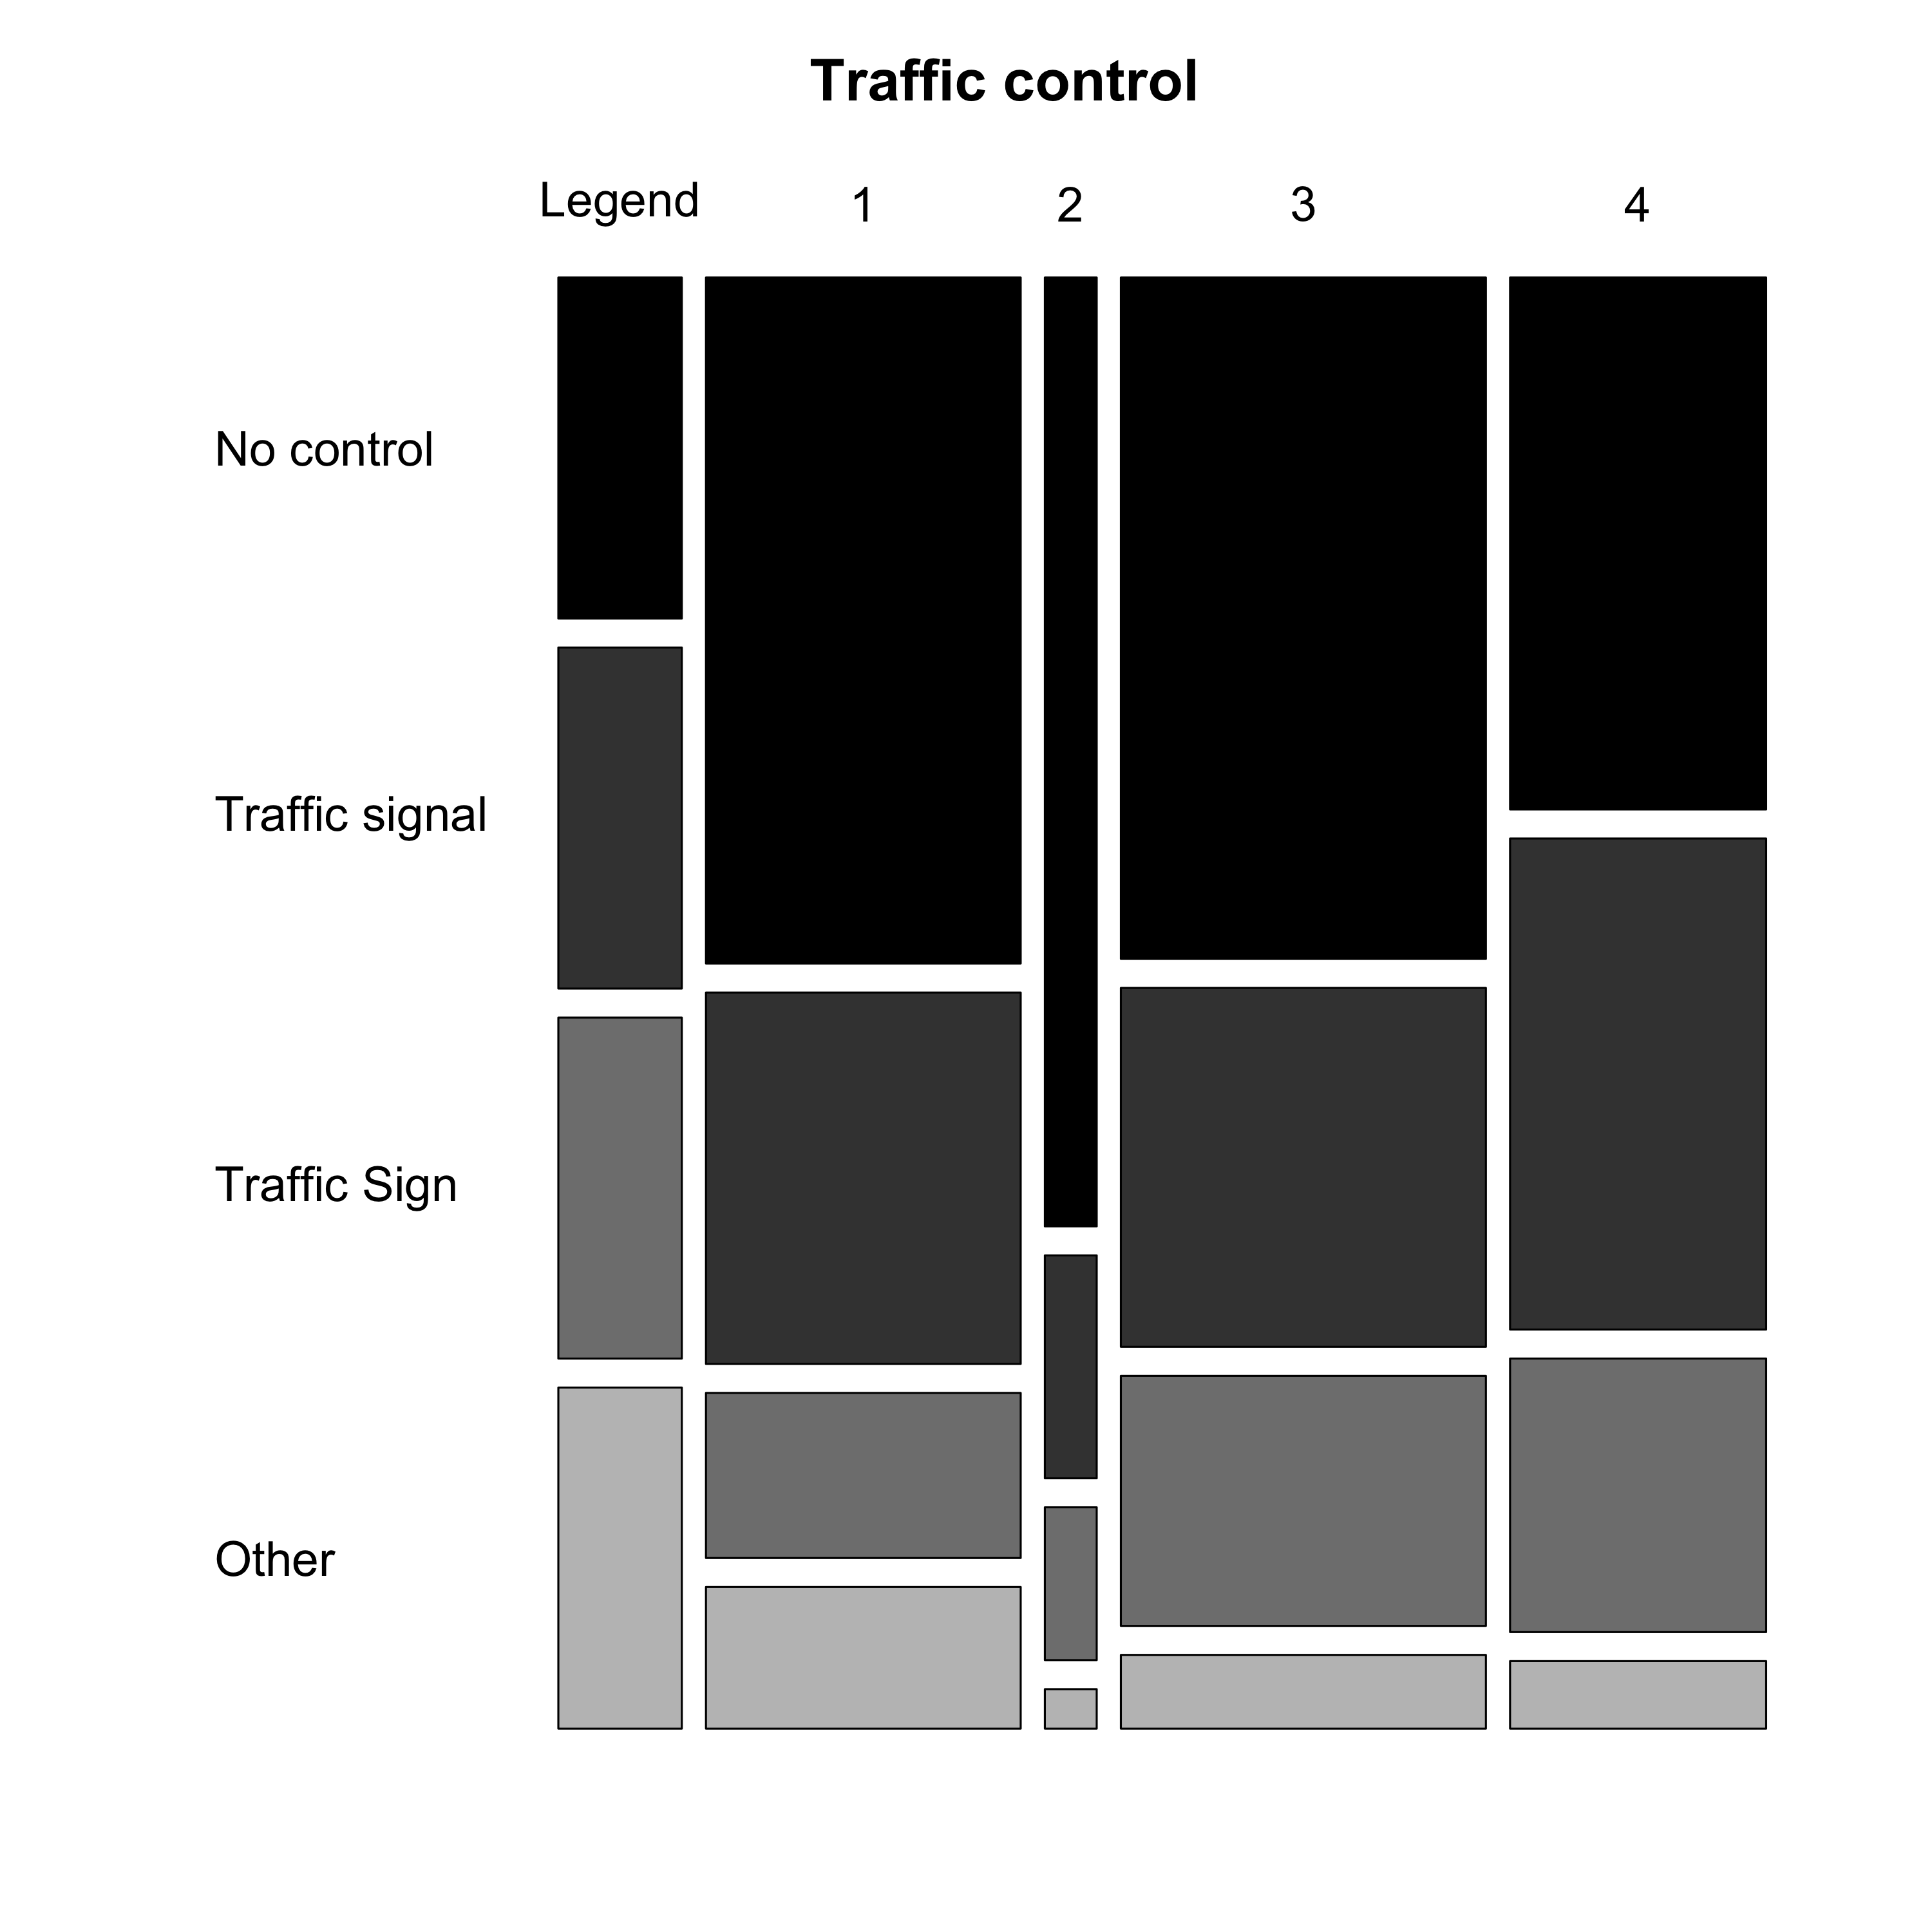
\includegraphics[width=1\linewidth]{traf_control_0509.png}
                \caption{2005--2009}
        \end{subfigure}%
        \begin{subfigure}{.5\textwidth}
%  \centering
                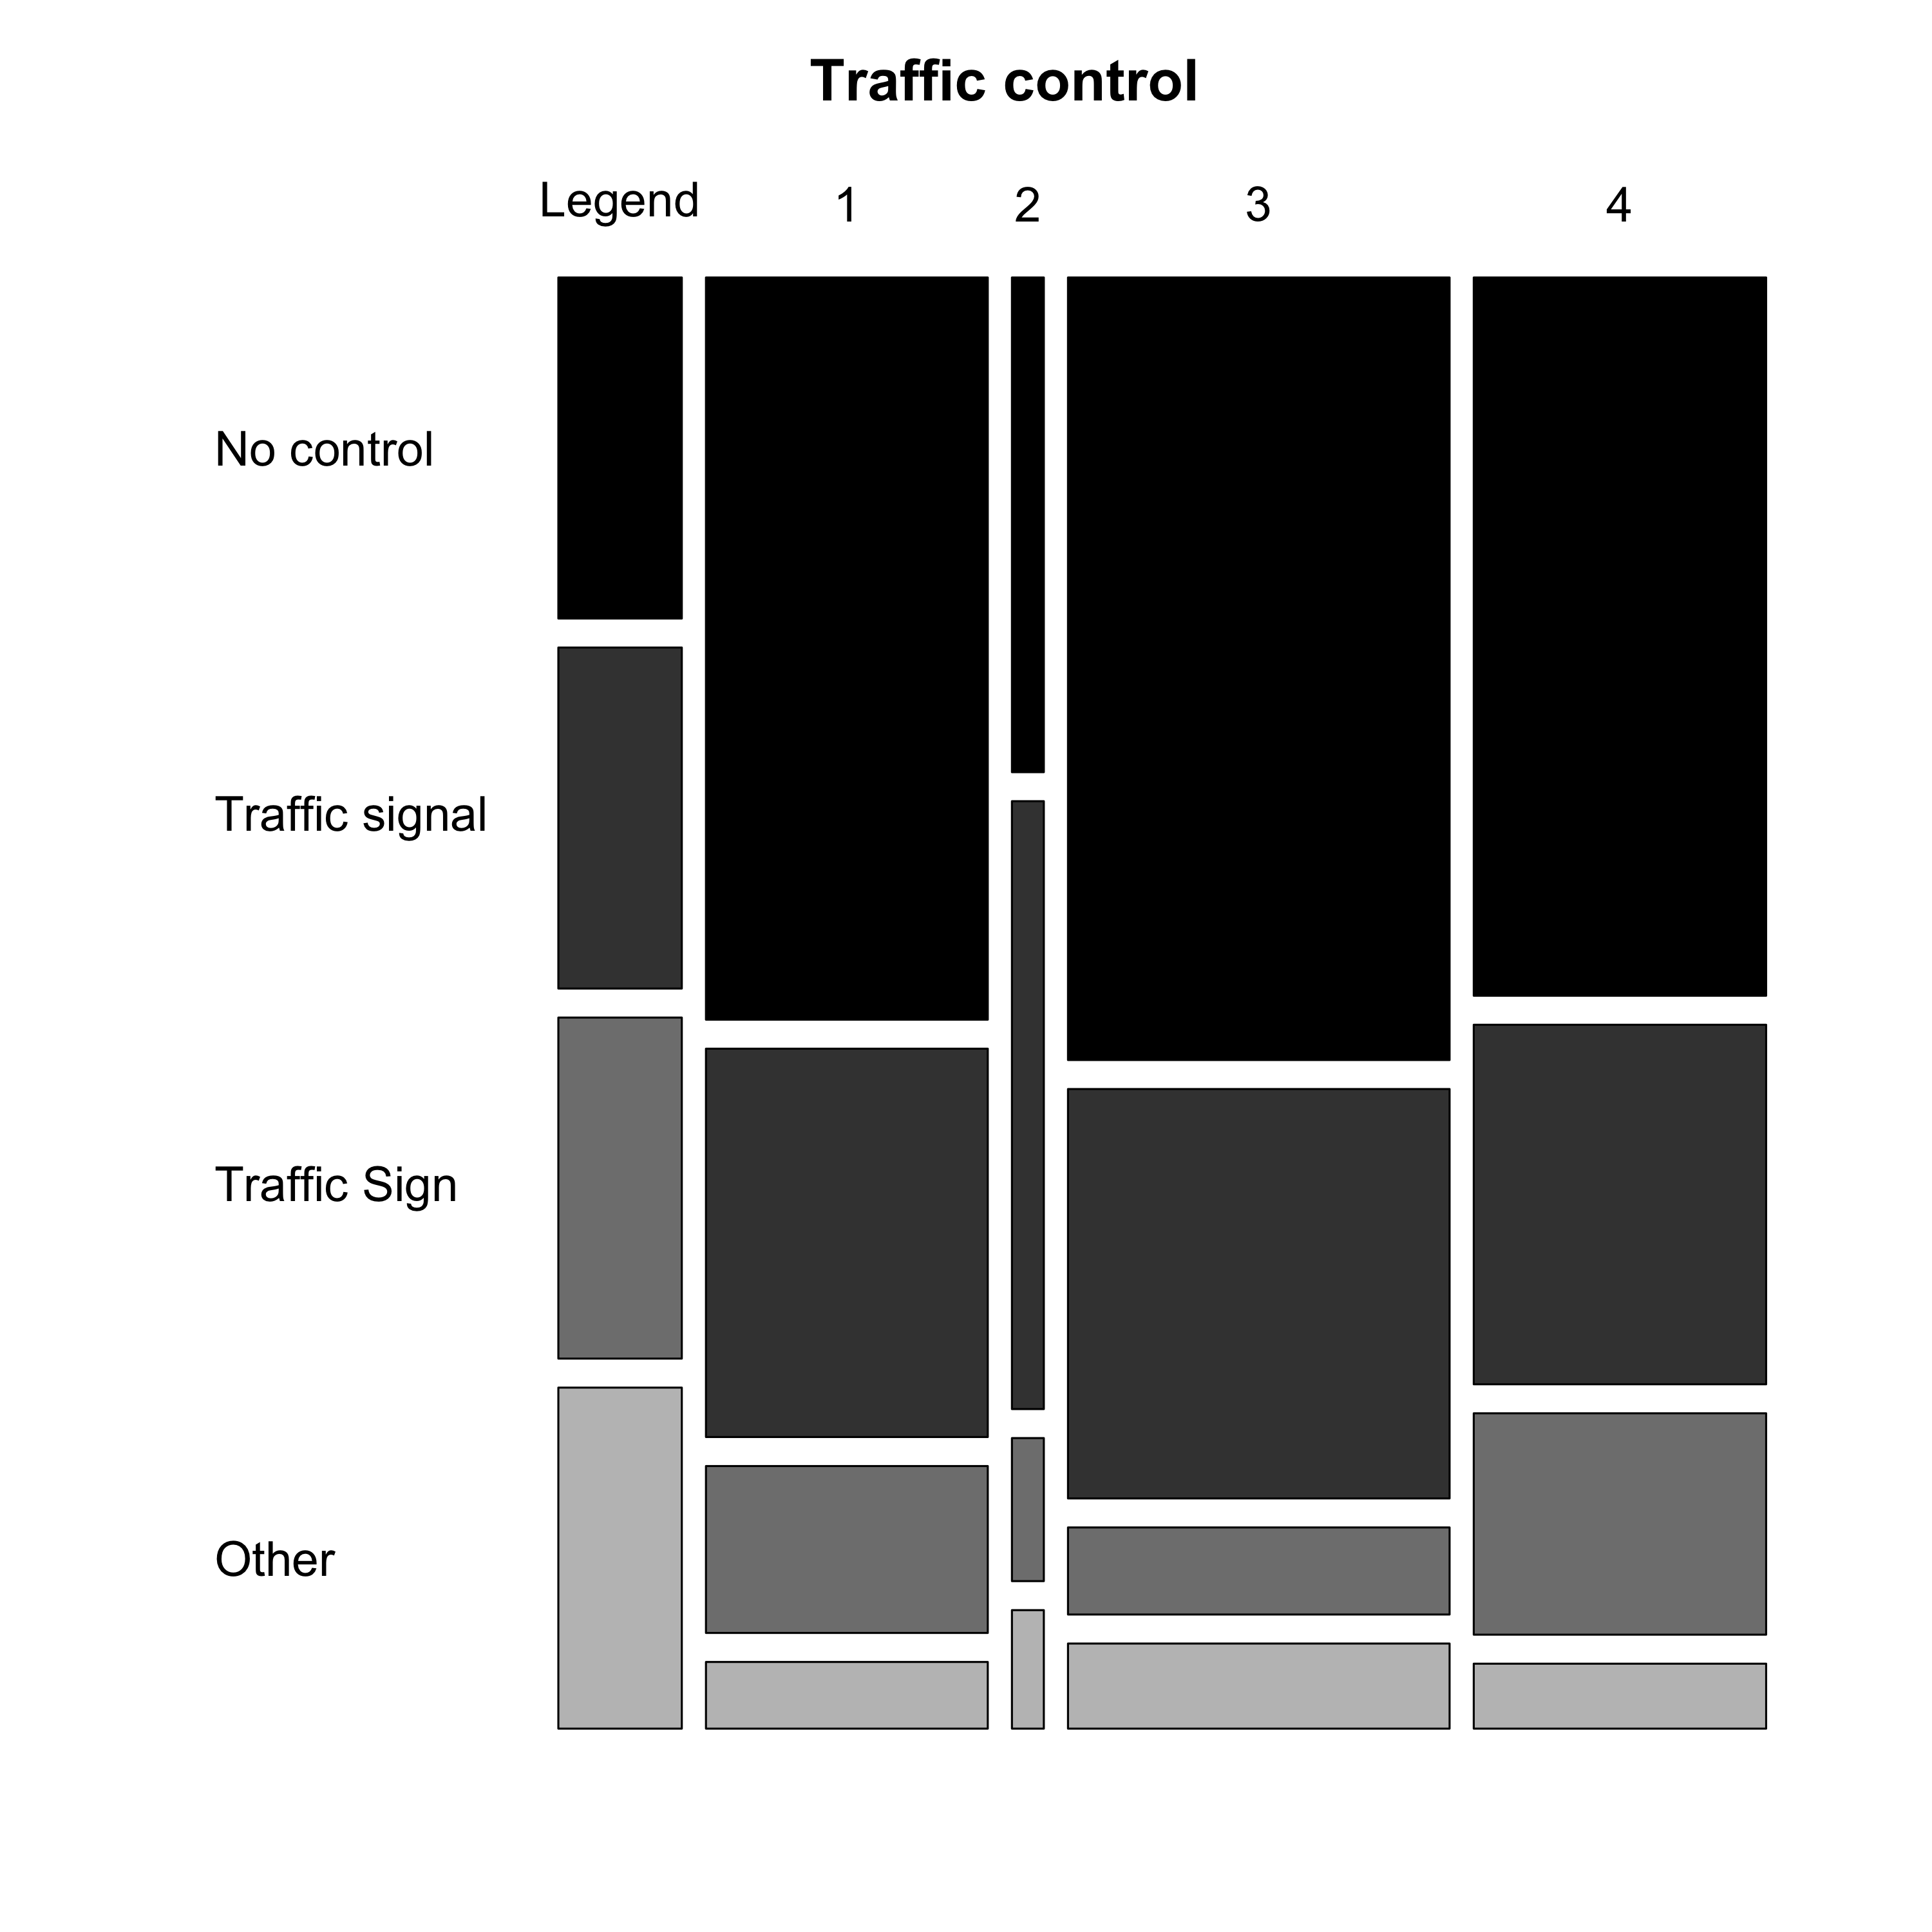
\includegraphics[width=1\linewidth]{traf_control.png}
                \caption{2010--2015}
        \end{subfigure}
        \caption{Mosaic plots giving the breakdown of the variable ``traffic control devices applicable to the bus at the time of the accident'' for each of the four clusters.}
        \label{fig:clus8}
\end{figure}
%%%%%%%%%%%%%%%%%%%%%%%%%%%%%%%%%%%%%%%%%%%%%%%%%%%%%%%%%%%%%%%%%%%%%%%%%%%%%%%%%%%%

%%%%%%%%%%%%%%%%%%%%%%%%%%%%%%%%%%%%%%%%%%%%%%%%%%%%%%%%%%%%%%%%%%%%%%%%%%%%%%%%%%%%
\begin{figure}[t]
%\centering
        \begin{subfigure}{.5\textwidth}
%  \centering
                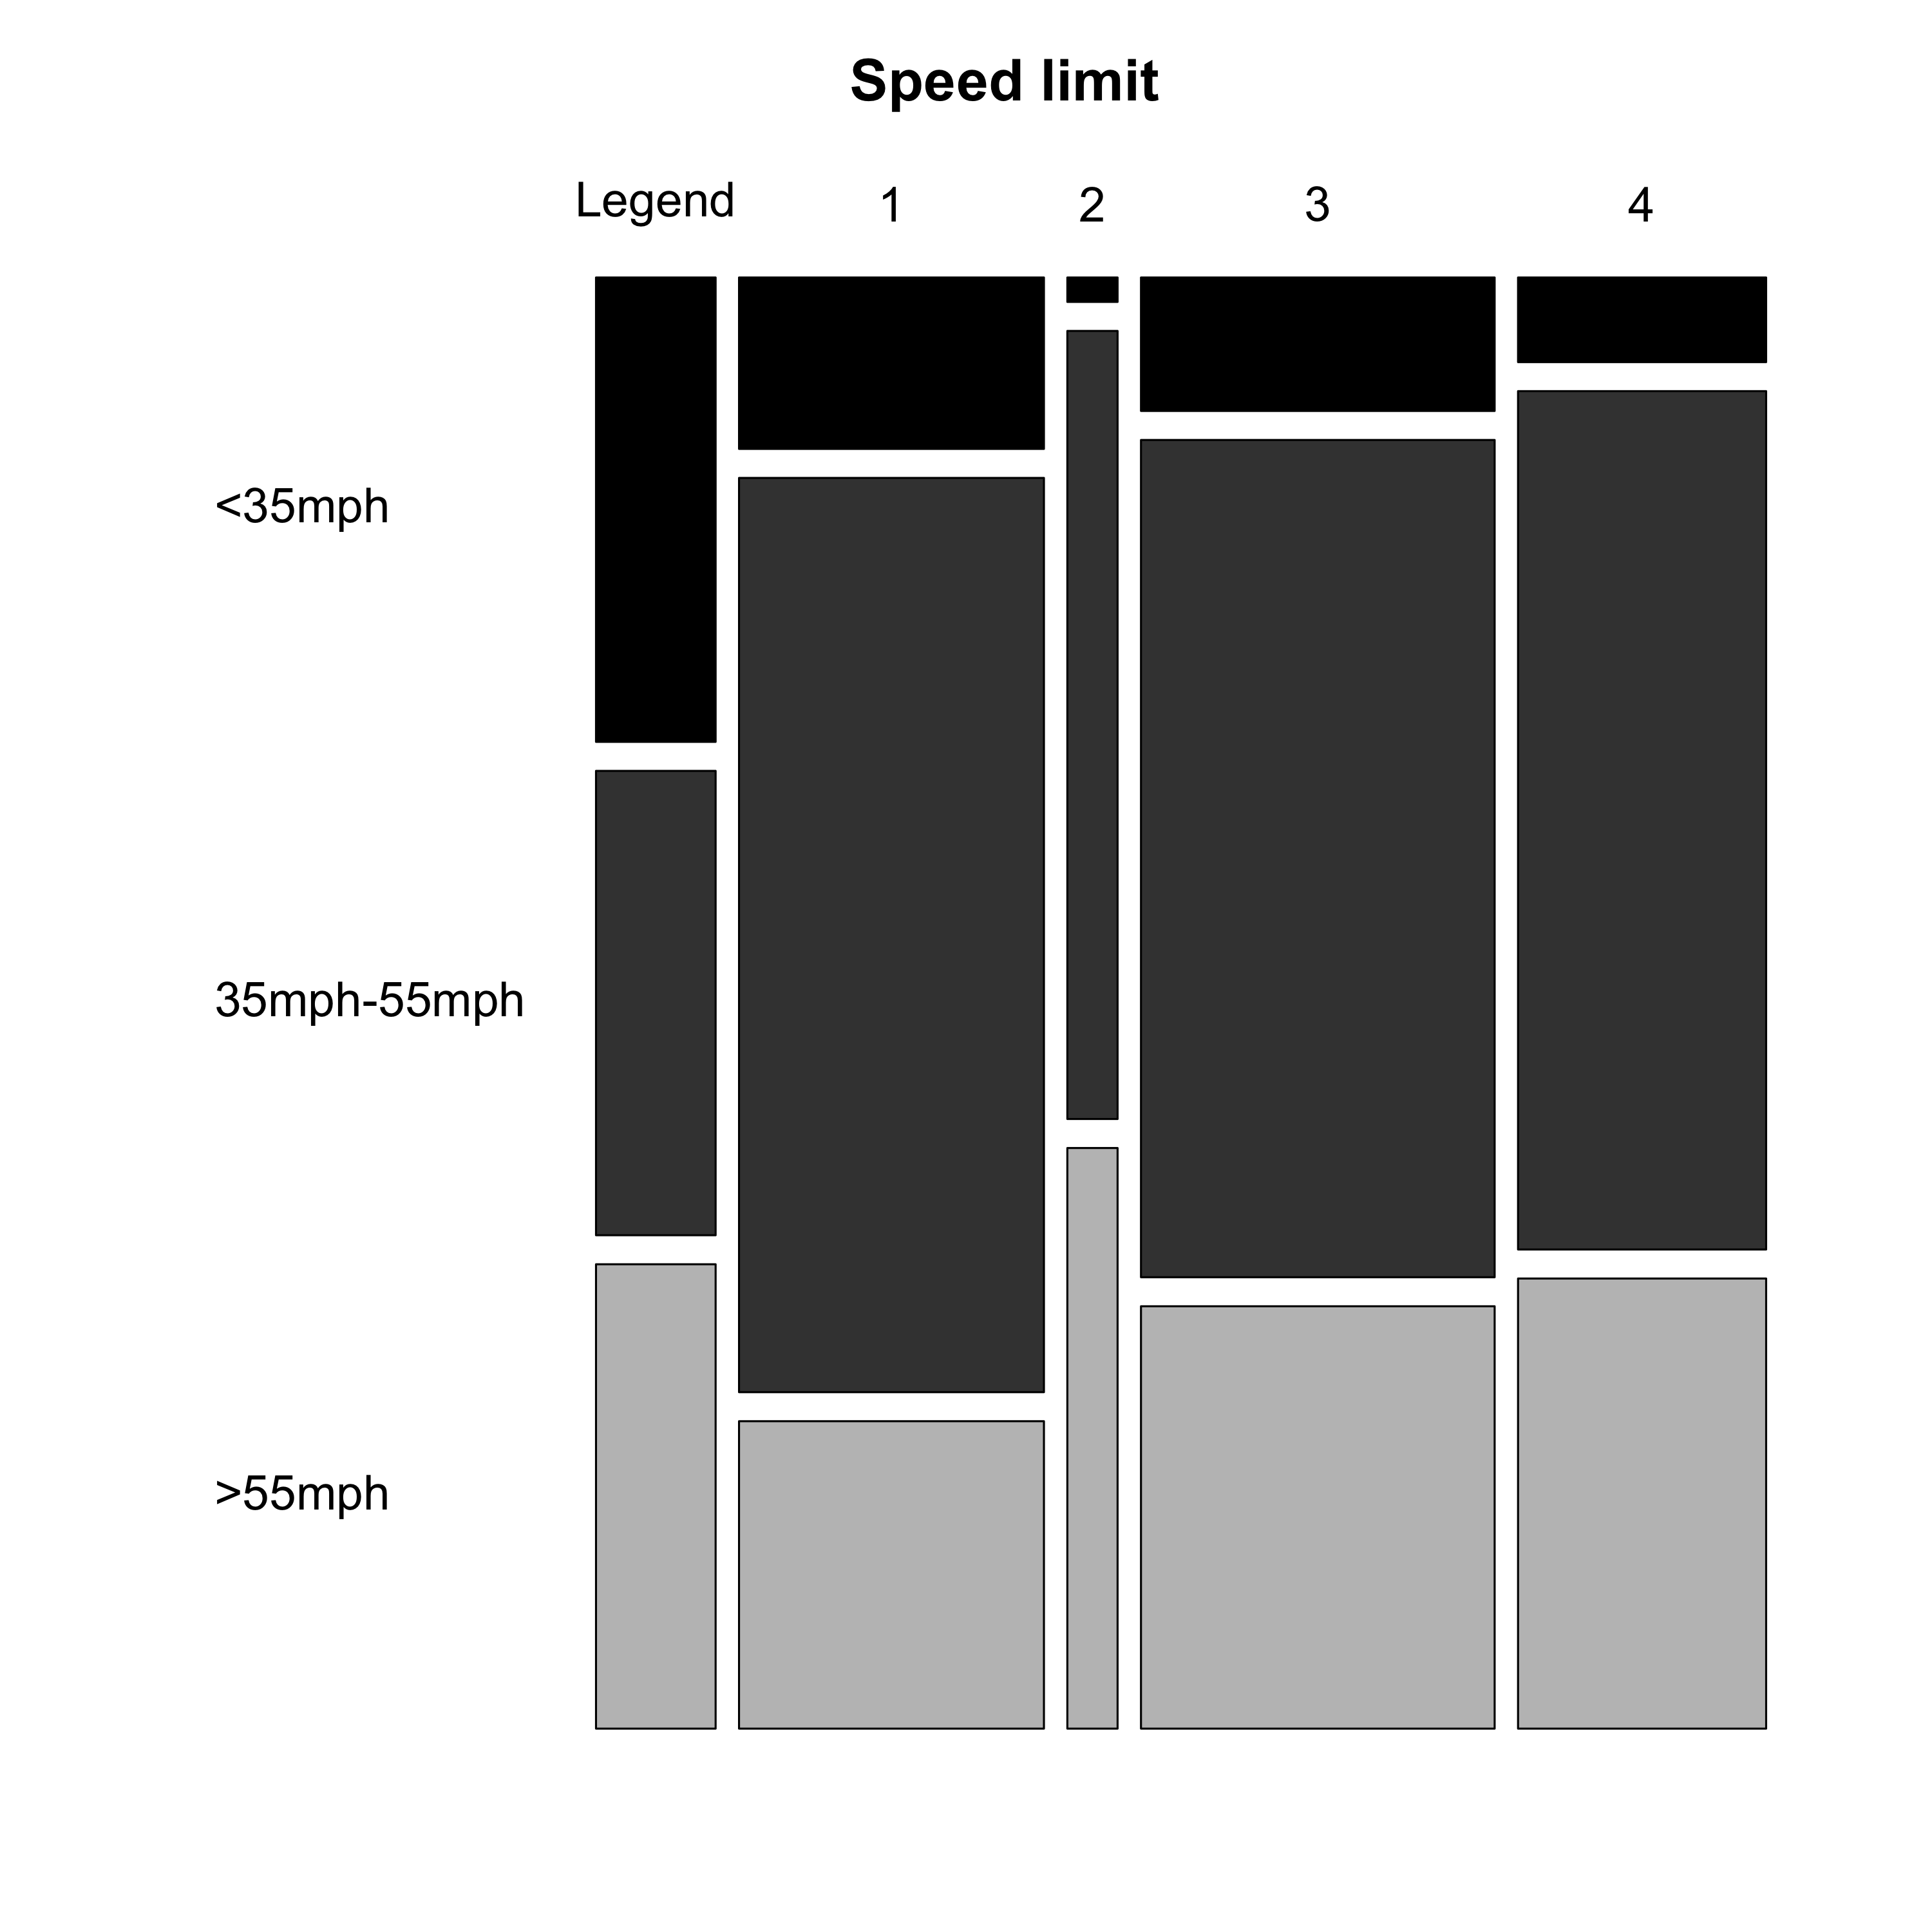
\includegraphics[width=1\linewidth]{spd_lim_0509.png}
                \caption{2005--2009}
        \end{subfigure}%
        \begin{subfigure}{.5\textwidth}
%  \centering
                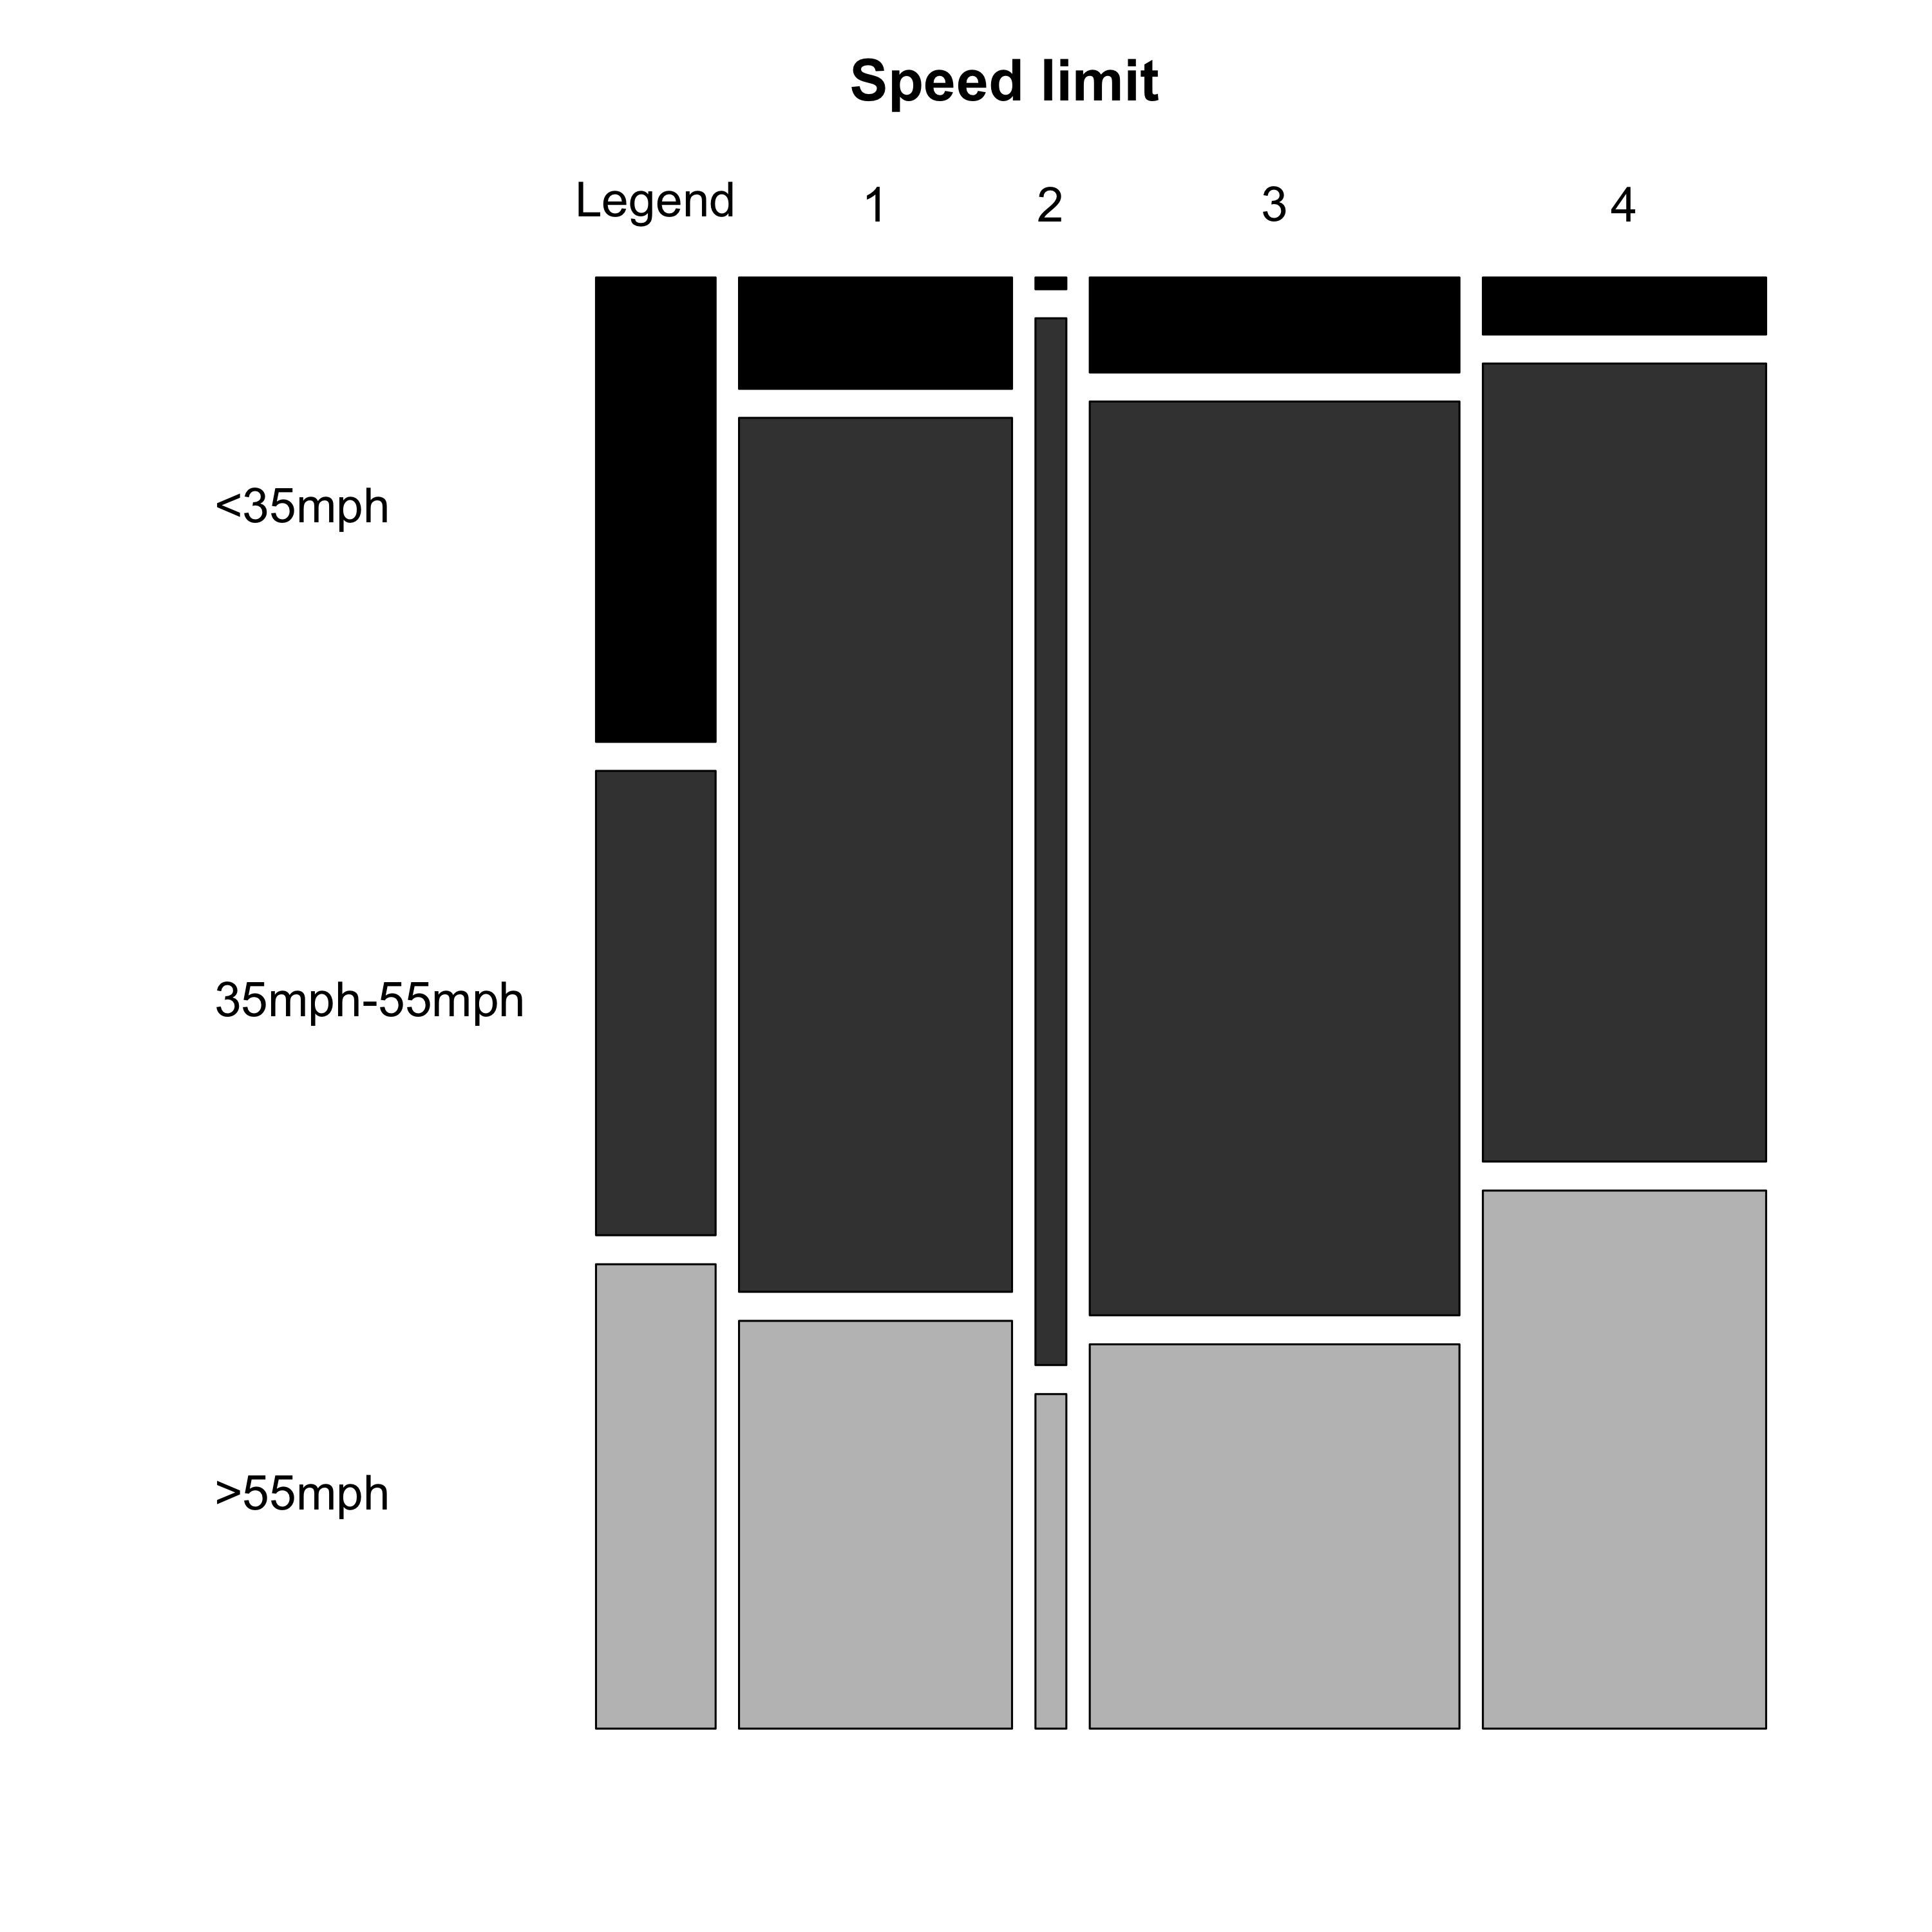
\includegraphics[width=1\linewidth]{spd_lim.png}
                \caption{2010--2015}
        \end{subfigure}
        \caption{Mosaic plots giving the breakdown of the variable ``speed limit of the traffic way where the accident occurred'' for each of the four clusters.}
 \label{fig:clus6}
\end{figure}
%%%%%%%%%%%%%%%%%%%%%%%%%%%%%%%%%%%%%%%%%%%%%%%%%%%%%%%%%%%%%%%%%%%%%%%%%%%%%%%%%%%%

%%%%%%%%%%%%%%%%%%%%%%%%%%%%%%%%%%%%%%%%%%%%%%%%%%%%%%%%%%%%%%%%%%%%%%%%%%%%%%%%%%%%
\begin{figure}[t]
%\centering
        \begin{subfigure}{.5\textwidth}
%  \centering
                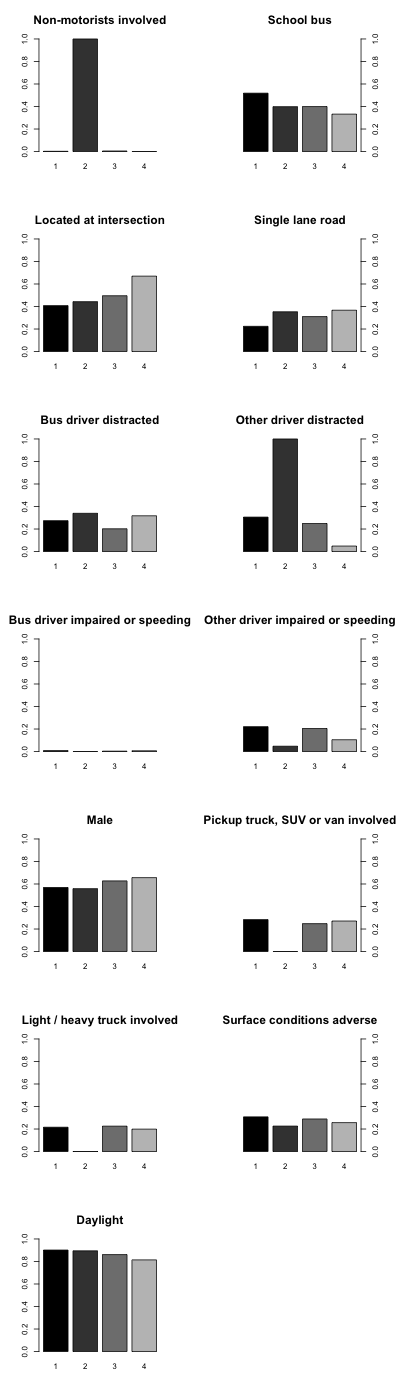
\includegraphics[width=1\linewidth]{binary_proportions_scaled_0509.png}
                \caption{2005--2009}
        \end{subfigure}%
        \begin{subfigure}{.5\textwidth}
%  \centering
                  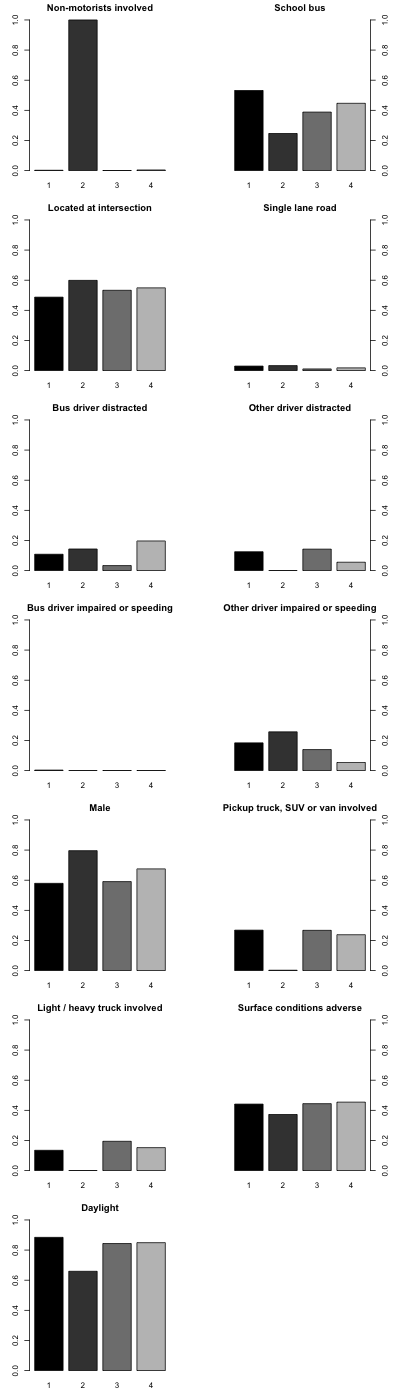
\includegraphics[width=1\linewidth]{binary_proportions_scaled.png}
                  \caption{2010--2015}
        \end{subfigure}
        \caption{Observed proportions for binary response variables for each of the four clusters.}
 \label{fig:clus2}
\end{figure}
%%%%%%%%%%%%%%%%%%%%%%%%%%%%%%%%%%%%%%%%%%%%%%%%%%%%%%%%%%%%%%%%%%%%%%%%%%%%%%%%%%%%

%%%%%%%%%%%%%%%
\begin{table}[t]
        \centering
        \caption{Taxonomy of crashes, 2005--2009.}
        \label{table:tax1}
        \resizebox{\textwidth}{!}{
        \begin{tabular}{@{}lllll@{}}
        \toprule
Characteristic                    & Cluster 1                       & Cluster 2                     & Cluster 3                    & Cluster 4 \\ \midrule
Single vs. Multiple vehicles      & {\color[HTML]{9A0000} Single}           & Multiple                        & Multiple                     & Multiple \\
(\textgreater85\%)                &                                 &                               &                              & \\ \midrule
Non-motorist involvement    & {\color[HTML]{680100} 100\%} 			  & 0\%                            & 0\%                        & 0\% \\ \midrule
Bus movement prior to crash       & going straight                        & going straight                & stopping              & turning left\\
                                  & (37.8\%)                        & (64.2\%),                     & (50.6\%),                      & (27.1\%),\\
                                  & turning right                   & stopping                  & going straight                    & going straight   \\
                                  &  (19.4\%)                       & (17.3\%),                  & (26\%)                     & (19.7\%),\\
                                  & parking                              &                        &   decelerating                           &other \\ 
                                  & (15.1\%)                            &                      &  (10.8\%)                             & (20.5\%)\\ \midrule
Critical event that made the      & vehicle turning   & other vehicle    & other vehicle         & vehicle  \\ 
crash imminent                    & (49.3\%)                 & encroaching      & in lane                   & turning\\
                                  & Non-motorist                  & into lane                &  (96.4\%)               & (90.7\%)  \\
                                  &  at fault                               & (92.1\%)            &                    &  \\
                                  &  (29\%)                              &                &                              & \\ \midrule
Bus driver distracted             & 35.8\%                  & 19.7\%     & 27.1\%           & 32.1\%  \\ \midrule
Other vehicle's driver or the     & {\color[HTML]{9A0000} 4.7\%}    & 21.0\%   & 23.0\%     & 10.5\% \\
non-motorist charged with         & & & & \\
alcohol/drug/impairment           & & & & \\
related offense                   & & & & \\ \midrule
Was a school bus involved?        &40.8\%  & 39.1\% & {\color[HTML]{9A0000} 51.7\%} & 35.4\%  \\ \midrule
Daylight condition - was          & 89.2\% & 86.6\% & 89.9\% & 81.7\%  \\
there sufficient light?           & & & & \\ \midrule
Did the accident happen           & 42.9\% & 50.3\% & 42.0\% & {\color[HTML]{9A0000} 63.0\%}  \\
at an intersection?               & & & & \\ \midrule
Bus driver gender (male?)         & 54.7\% & 62.8\% & 56.8\% & 65.3\%  \\ \midrule
Light/ heavy truck involvement    & 0.1\% &23.4\% & 21.5\% & 18.9\%  \\ \midrule
Was the other driver             & 0.1\% & 25.6\% & 31.0\% & {\color[HTML]{9A0000} 4.9\%}  \\
distracted?          & & & & \\ \midrule
Was there a pick-up truck/        & 0.0\% & 23.1\% & 27.6\% & 29.9\%  \\
van/ SUV involved?                & & & & \\ \midrule
Single lane vs. multiple lanes    &  2.5\% & 0.5\% & 1.6\% & 0.9\% \\ \bottomrule
        \end{tabular}
        }
\end{table}
%%%%%%%%%%%%%%%

The four clusters from the \textbf{2010--2015 dataset} can be
described as follows. Note that we have rearranged the arbitrary
ordering, so that the cluster number matches the corresponding cluster
from the 2005--2009 results. 

\noindent
\textbf{Cluster 1}: Single vehicle crashes involving non-motorists (100\%), (Figure \ref{fig:clus10} (b)), which mostly happened when the bus was going straight (37.7\%) or turning left/right (43.8\%) (Figure \ref{fig:clus6} (b)). There were two primary reasons for the crash: the bus was turning (23.5\%), or  the non-motorist was at fault (71.7\%) (Figure \ref{fig:clus12} (b)). In 14.3\% of the cases, the bus driver admitted to have been distracted, and 24.6\% of the time, a school bus was involved. 25.7\% of the incidents involved the non-motorist being impaired or under the influence. 59.8\% of the crashes happened at an intersection. 36.3\% of the crashes happened where the road had no traffic control, and in 44.4\% of the cases, there was a traffic signal (Figure \ref{fig:clus8} (b)). This was the cluster with the highest percentage of male drivers (79.3\%). 66.0\% of the crashes happened during the daytime.

\noindent
\textbf{Cluster 2}: Multi-vehicle crashes (93.3\% involving two vehicles) which mostly happened when the bus was going straight (66.8\%) or stopping (15.3\%). The crash was primarily due to the another vehicle trying to encroach into the bus' lane (96.3\%), implying that the crash was mainly the other driver's fault. In only  2.5\% of the cases did the bus driver admit to have been distracted, and 39.3\% of the time, a school bus was involved. Most of the crashes happened on roadways with moderate to high speed limits (64.8\% on roads with 35--55 MPH and 28.0\% on roads with greater than 55 MPH) (Figure \ref{fig:clus6} (b)). For 13.8\% of the crashes, at least one of the other drivers involved was distracted, and 13.9\% of the cases involved at least one of the other drivers being impaired or under the influence. 53.4\% of the crashes happened at an intersection. 57.8\% of the crashes happened where the road had no traffic control, in 30.2\% of the cases there was a traffic signal and in 6.0\% of the cases there was a traffic sign. 22.9\% of the cases involved a light or a heavy truck, and 26.6\% crashes involved an SUV, pickup truck, or van (Figure \ref{fig:clus2} (b)).

\noindent
\textbf{Cluster 3}:  Multi-vehicle crashes (90.0\% involving two vehicles, 10\% involving three or more vehicles), which happened largely due to the bus stopping (54.2\%) or going straight (25.6\%). The reason of the crash was mostly due to another vehicle being in the bus' lane (96.7\%), as observed in in the earlier dataset. 12.2\% of the time, the bus driver was distracted. In more than half the cases (55.1\%), a school bus was involved. Most of the crashes happened during the daytime (89.0\%). 50.0\% of the time, the crash happened when the bus was at an intersection. In 13.2\% of the cases, one of the other drivers were distracted, in 19.1\% of the cases, one of the other drivers were impaired or under the influence of alcohol or drugs. 15.7\% of the crashes involved a truck, but another 27.9\% of the crashes involved an SUV, pickup truck, or van. 63.2\% of the crashes happened on roads with speed limit between 35 and 55 MPH, and another 28.8\% happened on roads with speed limits greater than 55 MPH.  53.0\% of the crashes happened where the road had no traffic control, and in 29.2\% of the cases there was a traffic signal.\\
%%%%%%%%%%%%%%%%%%%%%%%%%%%%%%%%%%%%%%%%%%%%%%%%%%%%%%%%%%%%%%%%%%%%%%%%%%%%%%%%%%%%
\noindent
\textbf{Cluster 4}: Multi-vehicle crashes (98.7\% involving two vehicles) which mostly happened when the bus was going straight (23.2\%) or turning (43.0\%). The crash was primarily due to the bus trying to turn (85.5\%). In 19.0\% of the cases, the bus driver admitted to have been distracted, and 42.1\% of the time, a school bus was involved. Most of the crashes happened on roadways with moderate to high speed limits (57.9\% on roads with 35--55 MPH and 37.6\% on roads with greater than 55 MPH). In 5.5\% of the crashes, at least one of the other drivers involved was distracted, and only 5.0\% of the cases involved at least one of the other drivers being impaired or under the influence. 53.6\% of the crashes happened at an intersection. 53.2\% crashes happened where the road had no traffic control, and in 25.4\% of the cases, there was a traffic signal. 17.6\% cases involved a light or a heavy truck, and 22.9\% of the crashes involved an SUV, pickup truck, or van.\par
%%%%%%%%%%%%%%%%%%%%%%%%%%%%%%%%%%%%%%%%%%%%%%%%%%%%%%%%%%%%%%%%%%%%%%%%%%%%%%%%%%%%
\noindent
Table \ref{table:tax2} summarizes the characteristics of the 2010--2015 bus crash clusters.\par 
%\begin{table}[H]
%\centering
%\resizebox{\textwidth}{!}{%
%\begin{tabular}{lllll}
%\rowcolor[HTML]{C0C0C0} 
%\multicolumn{1}{c}{\cellcolor[HTML]{C0C0C0}\textbf{Attribute}} & \multicolumn{1}{c}{\cellcolor[HTML]{C0C0C0}\textbf{Cluster 1}} & \multicolumn{1}{c}{\cellcolor[HTML]{C0C0C0}\textbf{Cluster 2}} & \multicolumn{1}{c}{\cellcolor[HTML]{C0C0C0}\textbf{Cluster 3}} & \multicolumn{1}{c}{\cellcolor[HTML]{C0C0C0}\textbf{Cluster 4}} \\
%\begin{tabular}[c]{@{}l@{}}Single vs. Multiple vehicles\\ (\textgreater85\%)\end{tabular} & Multiple & {\color[HTML]{9A0000} Single} & Multiple & Multiple \\
%Non-motorist involvement & 0.1\% & {\color[HTML]{680100} 100\%} & 0.02\% & 0.3\% \\
%Bus movement prior to crash & {\color[HTML]{333333} \begin{tabular}[c]{@{}l@{}}Going straight\\ (66.4\%),\\ Stopping \\ (16\%)\end{tabular}} & {\color[HTML]{333333} \begin{tabular}[c]{@{}l@{}}Going straight \\ (37.9\%), overtaking\\  (27.1\%)\end{tabular}} & \begin{tabular}[c]{@{}l@{}}Going straight\\ (22.4\%), \\ Overtaking\\ (24.8\%)\end{tabular} & \begin{tabular}[c]{@{}l@{}}Stopping\\ (52.9\%), \\ going straight \\ (26.2\%)\end{tabular} \\
%\begin{tabular}[c]{@{}l@{}}Critical event that made the \\ crash imminent\end{tabular} & \begin{tabular}[c]{@{}l@{}}Encroaching in \\ another vehicle's \\ lane (95.6\%)\end{tabular} & \begin{tabular}[c]{@{}l@{}}Vehicle turning\\ (23.5\%), non-\\ motorist \\ encroaching into\\ lane (71.9\%)\end{tabular} & \begin{tabular}[c]{@{}l@{}}Vehicle \\ turning\\ (87.5\%)\end{tabular} & \begin{tabular}[c]{@{}l@{}}In another \\ vehicle's \\ lane (96.4\%)\end{tabular} \\
%Bus driver distracted & 10.8\% & 14.3\% & {\color[HTML]{9A0000} 3.2\%} & 19.6\% \\ \\
%\begin{tabular}[c]{@{}l@{}}Other vehicle's driver or the \\ non-motorist charged with \\ alcohol/drug/impairment \\ related offense\end{tabular} & 18.4\% & {\color[HTML]{9A0000} 25.7\%} & 13.9\% & 5.4\% \\
%Was a school bus involved? & {\color[HTML]{9A0000} 53.2\%} & 24.6\% & 38.8\% & 44.6\% \\ \\
%\begin{tabular}[c]{@{}l@{}}Daylight condition - was there\\ sufficient light?\end{tabular} & 88.4\% & {\color[HTML]{9A0000} 65.9\%} & 84.3\% & 84.9\% \\ \\
%\begin{tabular}[c]{@{}l@{}}Did the accident happen at an\\ intersection?\end{tabular} & 48.7\% & {\color[HTML]{9A0000} 59.9\%} & 53.3\% & {\color[HTML]{333333} 54.9\%} \\ \\
%Bus driver (male)? & 57.9\% & {\color[HTML]{9A0000} 79.6\%} & 59.1\% & 67.5\% \\ \\
%Light/ heavy truck involvement & {\color[HTML]{9A0000} 0\%} & {\color[HTML]{9A0000} 15.2\%} & 19.4\% & 13.4\% \\ \\
%\begin{tabular}[c]{@{}l@{}}Was the other driver/ \\ non motorist distracted?\end{tabular} & 0\% & {\color[HTML]{9A0000} 5.5\%} & 14.2\% & {\color[HTML]{333333} 12.5\%} \\ \\
%\begin{tabular}[c]{@{}l@{}}Was there a pick-up truck/ van/\\ SUV involved?\end{tabular} & 26.8\% & {\color[HTML]{9A0000} 0.2\%} & 26.7\% & {\color[HTML]{9A0000} 23.7\%} \\ \\
%Single lane vs. multiple lanes & {\color[HTML]{333333} 2.9\%} & 3.2\% & 1.6\% & 1.7\%
%\end{tabular}%
%}
%\caption{Taxonomy of crashes 2010 - 2015}
%\label{table:tax2}
%\end{table}

%%%%%%%%%%%%%%%
\begin{table}[t]
        \centering
        \caption{Taxonomy of crashes, 2010--2015.}
        \label{table:tax2}
        \resizebox{\textwidth}{!}{
        \begin{tabular}{@{}lllll@{}}
        \toprule
Characteristic                       & Cluster 1        & Cluster 2        & Cluster 3         & Cluster 4 \\ \midrule
Single vs. Multiple vehicles  & {\color[HTML]{9A0000} Single}     & Multiple  & Multiple   & Multiple \\
(\textgreater85\%)                &                   &                               &                              & \\ \midrule
Non-motorist involvement    & {\color[HTML]{680100} 100\%}   &0.3\%   & 0.3\%               & 11.2\% \\ \midrule
Bus movement prior to crash       & going straight        & going straight    & stopping                & turning left\\
                                                     & (37.7\%),               & (66.8\%),           & (54.2\%),                  & (24.4\%),\\
                                                     & turning left                & stopping         & going straight           & going straight    \\
                                                     & (27.0\%)                   & (15.3\%)          & (25.6\%)                   & (23.2\%)\\
                                                     &  turning right             &                         &                                  & turning right\\ 
                                                     & (16.8\%)                    &                         &                                  & (18.6\%)\\ \midrule
Critical event that made the      & non-motorist        & other vehicle                 & other vehicle         & vehicle  \\ 
crash imminent                         & at fault                  & encroaching into           & in lane                   & turning\\
                                                  & (71.7\%)               & lane (96.3\%),               &   (96.7\%)              & (85.5\%)  \\
                                                  &  vehicle turning     &                                      &                                &  \\
                                                  &  (23.5\%)               &                                      &                                   & \\ \midrule
Bus driver distracted                 & 14.3\%              & {\color[HTML]{9A0000} 2.5\%}         & 12.2\% & 19.0\%  \\ \midrule
Other vehicle's driver or the     & {\color[HTML]{9A0000} 25.7\%}        &13.9\%   & 19.1\%                       & 5.0\% \\
non-motorist charged with         & & & & \\
alcohol/drug/impairment           & & & & \\
related offense                   & & & & \\ \midrule
Was a school bus involved?      &24.6\%  & 39.3\% & {\color[HTML]{9A0000} 55.1\%} & 42.1\%  \\ \midrule
Daylight condition - was          & {\color[HTML]{9A0000} 66.0\%} & 84.2\%  & 89.0\% & 84.6\%  \\
there sufficient light?           & & & & \\ \midrule
Did the accident happen           & 59.8\% & 53.4\% & 50.0\% &  53.6\%  \\
at an intersection?               & & & & \\ \midrule
Bus driver gender (male?)         & 79.3\% & 58.2\% & 57.8\% & 68.6\%  \\ \midrule
Light/ heavy truck involvement    &  0.0\% &  22.9\% & 15.7\% & 17.6\%  \\ \midrule
Was the other driver            & 0.0\% &  13.8\% & 13.2\% & 5.5\%  \\
distracted?                           & & & & \\ \midrule
Was there a pick-up truck/        &0.2\%  & 26.6\%  & 27.9\% &  22.9\%  \\
van/ SUV involved?                & & & & \\ \midrule
Single lane vs. multiple lanes    &1.0\% & 1.0\% & 2.5\% & 1.3\% \\ \bottomrule
        \end{tabular}
        }
\end{table}
%%%%%%%%%%%%%%%
